\pdfoutput=1
%\documentclass[review,onefignum,onetabnum,final]{siamart171218}
\documentclass[review]{siamart171218}
%\documentclass{article}

%\usepackage{fullpage}
\usepackage{cite}
%\usepackage{geometry}

\usepackage{amsmath, amsfonts, amssymb}
\DeclareMathOperator*{\argmin}{\arg\,\min}
\DeclareMathOperator*{\argmax}{\arg\,\max}
\usepackage{algorithmic}

\newtheorem*{remark}{Remark}
\theoremstyle{assumption}
\newtheorem{assumption}{Assumption}

%\newtheorem{theorem}{Theorem}
%\newtheorem{remark}{Remark}
%\newenvironment{proof}{\paragraph{Proof:}}{\hfill$\square$}
%\newtheorem{assumption}{Assumption}
%\newtheorem{lemma}{Lemma}

\usepackage{hyperref}
\usepackage[titletoc,toc,title]{appendix}
\usepackage{tikz}
%\usepackage{hhline}
\usepackage{graphicx, color, bm}
\usepackage{subfig}
\usepackage{pgfplots}
\usepackage{pgfplotstable}
\usepackage{slopetri} % my own package for drawing triangle slopes

\renewcommand{\hat}{\widehat}
\renewcommand{\tilde}{\widetilde}

%% d in integrand
\newcommand*\diff[1]{\mathop{}\!{\mathrm{d}#1}}
\newcommand{\diag}[1]{{\rm diag}\LRp{#1}}
\newcommand{\td}[2]{\frac{{\rm d}#1}{{\rm d}{\rm #2}}}
\newcommand{\pd}[2]{\frac{\partial#1}{\partial#2}}
\newcommand{\nor}[1]{\left\| #1 \right\|}
\newcommand{\LRp}[1]{\left( #1 \right)}
\newcommand{\LRs}[1]{\left[ #1 \right]}
\newcommand{\LRa}[1]{\left\langle #1 \right\rangle}
\newcommand{\LRb}[1]{\left| #1 \right|}
\newcommand{\LRc}[1]{\left\{ #1 \right\}}
\newcommand{\LRceil}[1]{\left\lceil #1 \right\rceil}
\newcommand{\LRl}[1]{\left. #1 \right|}
\newcommand{\pdn}[3]{\frac{\partial^{#3}#1}{\partial#2^{#3}}}
\newcommand{\Grad} {\ensuremath{\nabla}}
\newcommand{\jump}[1] {\ensuremath{\llbracket#1\rrbracket}}
\newcommand{\avg}[1] {\ensuremath{\LRc{\!\{#1\}\!}}}

\newcommand{\note}[1]{{\color{blue}{#1}}}

\graphicspath{{./figs/}}


%%%%%%%%%%%%%%%%%%%%%%%%%%%%%%%%%%%%%%%%%%%%%%%%%%%%%%%%%%%%%%%
%%%%%%%%%%%%%%%%%%%%%%%%%%%%%%%%%%%%%%%%%%%%%%%%%%%%%%%%%%%%%%%
%%%%%%%%%%%%%%%%%%%%%%%%%%%%%%%%%%%%%%%%%%%%%%%%%%%%%%%%%%%%%%%

\date{}
\author{Jesse Chan}
\title{Entropy stable reduced order modeling of nonlinear conservation laws}

\begin{document}

\maketitle

\begin{abstract}
Reduced order models of nonlinear conservation laws in fluid dynamics do not typically inherit stability properties of the full order model. We discuss the construction of reduced models of nonlinear conservation laws which retain accuracy while inheriting a semi-discrete entropy inequality independently of discretization resolutions and parameters. 
\end{abstract}

\tableofcontents

%\begin{itemize}
%\item Intro
%\item Entropy conservation for FOM
%\item Entropy conservation for POD
%\item Entropy stability via entropy dissipation
%\item Entropy stable hyper-reduction
%\item Proof: accuracy of projected operator
%\item Proof: entropy stability for periodic domain
%\item Proof: conservation if $\bm{1}$ is contained in $\bm{V}_r$
%\item Non-periodic domains and constrained hyper-reduction

%\item Numerical experiments
%\begin{itemize}
%\item Singular values of conservative snapshots vs conservative + entropy variable snapshots.
%\item 1D experiments, shocks, error convergence plots
%\item Effect of different hyper-reduction techniques (optimizing for $V_{\rm test} V_{\rm test}$ and $V_r V_{\rm test}$ vs $V_r V_r$)
%\item Comparison of entropy stable viscosity vs regular hyper-reduced viscosity
%\item Comparison of snapshots from entropy stable FOM vs regular FOM.  
%\item 2D experiments: KH and acoustic pulse
%\end{itemize}
%\end{itemize}

\section{Introduction}

Projection-based model reduction constructs low-dimensional surrogate models for many-query scenarios (e.g., simulations over multiple parameter values) that can be evaluated over a range of parameters at a low \textit{online} cost in exchange for a more expensive \textit{offline} pre-computation step \cite{benner2015survey}.  %Reduced order models (ROMs) can be constructed, for example, by performing a Galerkin projection of the original full order model onto a reduced basis.  
The development of reduced order models (ROMs) is relatively mature for several classes of problems (e.g., linear time-invariant systems, coercive elliptic PDEs).  However, the construction of robust and stable ROMs for transient and convection-dominated problems remains an active area of research \cite{cagniart2019model}.  

For certain PDEs, ``structure-preserving'' ROMs provide robustness and stability by preserving energetic properties of the full system at the discrete level.  ROMs which retain either Lagrangian \cite{lall2003structure, carlberg2015preserving} or Hamiltonian structure \cite{polyuga2010structure, benner2012interpolation, gugercin2012structure, peng2016symplectic, chaturantabut2016structure, gong2017structure, afkham2017structure, afkham2018structure} have been constructed by combining Galerkin projection with an appropriate formulation of the full order model, and similar energy-conserving ROMs have been constructed for the incompressible Navier-Stokes equations \cite{farhat2014dimensional, farhat2015structure}.  The construction of structure-preserving ROMs to nonlinear conservation laws in fluid flow, however, remains an open problem.  For example, Galerkin projection yields ROMs which become unstable as the number of reduced basis functions (modes) is increased \cite{bui2007goal, carlberg2013gnat}.  As a result, stabilized discretizations are often employed.  Petrov-Galerkin ROMs, which use an alternative test basis \cite{maday2002blackbox, rozza2007stability, bui2007goal, amsallem2012stabilization, rozza2013reduced, ballarin2015supremizer, carlberg2017galerkin}, are a popular alternative, as are additional residual-based stabilization or dissipation terms \cite{wang2012proper, kalashnikova2014stabilization, caiazzo2014numerical, balajewicz2016minimal}.  Such models improve robustness in practice, though they do not provide a theoretical foundation for stability.  

The construction of stable ROMs for the compressible Navier-Stokes equations is complicated by their complex structure.  Thus, practitioners often develop structure-preserving entropy stable ROMs for simplifications of the underlying PDE (such as the time-dependent \textit{linearized} compressible Navier-Stokes equations \cite{barone2009stable, kalashnikova2010stability, serre2012reliable, amsallem2012stabilization, kalashnikova2014construction}) and extrapolate such models to the full nonlinear equations.  A promising alternative is to enforce physical conditions such as such as kinetic energy preservation, which are empirically related to stability \cite{maboudi2018conservative}.  These methods significantly improve the robustness of numerical methods in practice, and can guarantee a discrete entropy inequality for systems of nonlinear conservation laws which yield stable split formulations \cite{fisher2013discretely}.  

The approach taken in this work differs in the treatment of nonlinear terms.  In \cite{maboudi2018conservative}, equations are rewritten such that the nonlinear terms involve only polynomial (quadratic and cubic) nonlinearities, which can be evaluated exactly using precomputed matrices.  In this work, we approximate nonlinear terms using hyper-reduction techniques based on empirically computed quadrature rules \cite{an2008optimizing, hernandez2017dimensional}.  The hyper-reduction approach incurs approximation error; however, it is allows for the generalization of the split forms in \cite{maboudi2018conservative} to nonlinearly entropy stable formulations.

%
%Hyper-reduction methods
%\begin{itemize}
%\item Interpolatory: DEIM and QR-DEIM \cite{chaturantabut2010nonlinear, drmac2016new}, gappy POD \cite{bui2004aerodynamic, carlberg2011efficient}
%\item Element-based approaches: ECSW \cite{farhat2014dimensional, farhat2015structure}, EQP \cite{ryu2015extensions, yano2019lp, patera2017lp}
%\item Empirical cubature: \cite{an2008optimizing, hernandez2017dimensional}.  
%\end{itemize}
%
%Structure-preserving ROMs: 
%\begin{itemize}
%\item Linear Hamlitonian \cite{beattie2009interpolatory} 
%\item Nonlinear Hamiltonian systems: Gugercin \cite{gugercin2012structure}, Carlberg \cite{carlberg2015preserving}, Chaturantabut \cite{chaturantabut2016structure}, Gong \cite{gong2017structure}, Afkham et al.\ \cite{afkham2017structure, afkham2018structure}
%\item Conservation through explicit constraints over sub-meshes \cite{carlberg2017structure, carlberg2018conservative}
%\end{itemize}

In this work, we directly constructing entropy stable ROMs for nonlinear conservation laws through a modified Galerkin projection of an appropriate full order model.  The approach taken in this paper combines techniques from entropy stable finite volume schemes \cite{tadmor1987numerical, tadmor2003entropy} and entropy stable summation-by-parts (SBP) discretizations \cite{fisher2013high, carpenter2014entropy, chen2017entropy, crean2018entropy, chan2017discretely, chan2018discretely, chan2019skew} to produce entropy stable reduced order models.  The paper is organized as follows.  Section~\ref{sec:1} discusses the entropy inequality associated with systems of nonlinear conservation laws.  Section~\ref{sec:2} introduces a full order model on 1D periodic domains based on entropy stable finite volume schemes.  Section~\ref{sec:3} describes how to construct an entropy stable reduced basis approximation, while Section~\ref{sec:4} discusses entropy stable hyper-reduction techniques to reduce costs associated with the evaluation of nonlinear terms.  Section~\ref{sec:6} describes how to extend the aforementioned approaches to non-periodic boundary conditions, and Section~\ref{sec:7} describes the extension to higher dimensions.  We conclude in Section~\ref{sec:8} with numerical experiments verifying theoretical results.

\section{Entropy inequalities for nonlinear conservation laws}
\label{sec:1}
Let $\Omega$ denote some domain with boundary $\partial \Omega$.  General nonlinear conservation laws are expressed as a system of partial differential equations (PDEs) 
\begin{equation}
\pd{\bm{u}}{t}  + \sum_{i=1}^d\pd{\bm{f}_i(\bm{u})}{x_i} = 0, \qquad 
S(\bm{u}) \text{ is a convex function}, \qquad
\bm{v}(\bm{u}) = \pd{S}{\bm{u}},
\label{eq:nonlineqs}
\end{equation}
where $\bm{u}\in \mathbb{R}^n$ are the conservative variables, $\bm{f}_j$ are nonlinear fluxes, and $\bm{v}(\bm{u})$ are the \textit{entropy variables}.  By multiplying (\ref{eq:nonlineqs}) by the entropy variables, viscosity solutions \cite{oleinik1957discontinuous, kruvzkov1970first}  of popular fluid systems (e.g., shallow water, compressible Euler and Navier-Stokes \cite{hughes1986new, chen2017entropy}) can be shown to satisfy 
\begin{equation}
\int_{\Omega}\pd{S(\bm{u})}{t}\diff{\bm{x}} + \int_{\partial \Omega} \LRp{\bm{v}^T\bm{f}(\bm{u}) - \psi_i(\bm{u})}n_i \leq 0\label{eq:entropyineq},
\end{equation}
where $n_i$ denotes the $i$th component of the outward normal vector.  
The entropy inequality (\ref{eq:entropyineq}) is the analogue of energy stability for nonlinear conservation laws \cite{mock1980systems, harten1983symmetric}.  
However, due to the use of inexact treatment of nonlinear terms (e.g., from collocation approximations, aliasing errors, or inexact quadrature rules), most numerical methods for nonlinear conservation laws do not satisfy a discrete analogue of this stability condition. 

\section{The full order model: entropy stable finite volume schemes}
\label{sec:2}

The reduced order models in this work are constructed using full order models constructed from discretely entropy stable finite volume methods \cite{tadmor1987numerical}.  For simplicity, we illustrate the construction of full and reduced order models on a periodic 1D domain.  We note that, while the reduced order model will be constructed from an entropy stable scheme, the solution snapshots do not need to be generated by entropy stable full order model.  Throughout this work, we will assume that the both full and reduced models yield ``physically relevant'' solutions, such that the entropy is a convex function.  For example, for the compressible Euler and Navier-Stokes equations, we will assume that the thermodynamic variables (density and energy/temperature/pressure) are positive.  Guaranteeing both positivity and accuracy of numerical solutions for general discretizations remains challenging \cite{guermond2016invariant, guermond2019invariant}, and will be explored in future work.

A key ingredient of the full and reduced order models considered in this work are \textit{entropy conservative} numerical fluxes.  Let $\bm{u}_L, \bm{u}_R$ denote left and right states.  Then, a two-point numerical flux $\bm{f}_S(\bm{u}_L, \bm{u}_R)$ is entropy conservative if it satisfies the following three conditions
\begin{gather}
\bm{f}_S(\bm{u},\bm{u}) = \bm{f}(\bm{u}), \qquad \text{(consistency)} \label{eq:esflux}\\
\bm{f}_S(\bm{u}_L,\bm{u}_R) = \bm{f}_S(\bm{u}_R,\bm{u}_R), \qquad \text{(symmetry)} \nonumber\\
\LRp{\bm{v}_L-\bm{v}_R}^T\bm{f}_S(\bm{u}_L,\bm{u}_R) = \psi(\bm{u}_L) - \psi(\bm{u}_R), \qquad \text{(entropy conservation)}\nonumber,
\end{gather}
Let the domain be decomposed into $K$ cells of size $\Delta x$, and let ${\LRp{\bm{u}_h}_i}$ denote the vector containing mean values of the conservation variables over the $i$th cell.  An entropy conservative finite volume method results from discretizing the integral form of the conservation law as follows
\begin{align}
&\td{{\LRp{\bm{u}_h}_1}}{t} + \frac{\bm{f}_S({\LRp{\bm{u}_h}_2},\LRp{\bm{u}_h}_1)-\bm{f}_S({\LRp{\bm{u}_h}_1},{\LRp{\bm{u}_h}_K})}{\Delta x} = \bm{0}, \label{eq:nonlineqs1d}\\
&\td{{\LRp{\bm{u}_h}_i}}{t} + \frac{\bm{f}_S({\LRp{\bm{u}_h}_{i+1}},\LRp{\bm{u}_h}_i)-\bm{f}_S({\LRp{\bm{u}_h}_i},{\LRp{\bm{u}_h}_i-1})}{\Delta x} = \bm{0}, \qquad 1 < i < K \nonumber\\
&\td{{\LRp{\bm{u}_h}_K}}{t} + \frac{\bm{f}_S({\LRp{\bm{u}_h}_1},\LRp{\bm{u}_h}_K)-\bm{f}_S({\LRp{\bm{u}_h}_K},{\LRp{\bm{u}_h}_K-1})}{\Delta x} = \bm{0},\nonumber
\end{align}
where periodicity is imposed through the equations for ${\LRp{\bm{u}_h}_1}, {\LRp{\bm{u}_h}_K}$.  

We first rewrite the system (\ref{eq:nonlineqs1d}) in a matrix form which will be more amenable to model reduction.  We define the skew-symmetric matrix $\bm{Q}$ and flux matrix $\bm{F}$ such that
\begin{equation}
\bm{Q} = \frac{1}{2}\begin{bmatrix}
0 & 1 & &\ldots & -1\\
-1 & 0 & 1 &&  \\
& -1 & 0 & 1 &  \\
 & & & \ddots &  \\
1 & &\ldots  & -1 & 0
\end{bmatrix}, \qquad \bm{F}_{ij} = \bm{f}_{S}\LRp{\LRp{\bm{u}_h}_i, \LRp{\bm{u}_h}_j}.
\label{eq:Qmat}
\end{equation}
Note that $\bm{Q}\bm{1} = \bm{0}$, the matrix $\bm{F}$ is symmetric due to flux symmetry, and the diagonal of $\bm{F}$ is equal to $\bm{f}(\bm{u})$ due to flux consistency.  For a scalar nonlinear conservation law, the matrix-based formulation of (\ref{eq:nonlineqs1d}) is then equivalent to
\begin{align}
\Delta x \td{\bm{u}_h}{t} + 2\LRp{{\bm{Q}}\circ \bm{F}}\bm{1} = \bm{0}.
\label{eq:es}
\end{align}
where $\circ$ denotes the Hadamard product, $\bm{1}$ denotes the vector of all ones, and each entry of $\bm{u}_h$ corresponds to a point $\bm{x}_i$ in the domain.  In this setting, $\bm{Q}\circ\bm{F}$ extracts and takes linear combinations of nonlinear flux interactions between different nodal values of $(\bm{u}_h)_i$ and $(\bm{u}_h)_j$.  The discretization of the nonlinear flux term using $\LRp{\bm{Q}\circ \bm{F}}\bm{1}$ is commonly referred to as \textit{flux differencing} \cite{carpenter2014entropy, gassner2016split, chen2017entropy, crean2018entropy, chan2017discretely}.\footnote{The factor of 1/2 present in the definition of $\bm{Q}$ is to make (\ref{eq:es}) consistent with the entropy stable SBP literature.  The factor of 2 in (\ref{eq:es}) can also be derived from the chain rule \cite{chen2017entropy, crean2018entropy}.  }

For a system of $n$ nonlinear conservation laws, all matrices are treated in a Kronecker product fashion.  Let the vector $\bm{u}_h$ now correspond to the concatenated vector of components of the solution $\bm{u}_h = [\bm{u}_h^1, \ldots, \bm{u}_h^n]$.  Then, the matrix formulation of (\ref{eq:nonlineqs1d}) is given by
\begin{gather*}
\Delta x\td{\bm{u}_h}{t} + \LRp{\LRp{\bm{I}_{n \times n} \otimes \bm{Q} }\circ \bm{F}}\bm{1} = \bm{0},\\
\bm{F} = \begin{bmatrix}
\bm{F}_{1} & &\\
& \ddots &\\
&& \bm{F}_{n} \\
\end{bmatrix}, \qquad 
\LRp{\bm{F}_{i}}_{jk} = \bm{f}_{i,S}\LRp{\LRp{\bm{u}_h}_j, \LRp{\bm{u}_h}_k}.
\label{eq:essys}
\end{gather*}
Here, $\bm{F}$ is a block diagonal matrix where the $i$th block corresponds to the evaluation of the $i$th component of the numerical flux $\bm{f}_{i,S}(\bm{u}_L,\bm{u}_R)$.  From this point on, we drop explicit references to the Kronecker product to simplify notation, so that (\ref{eq:es}) applies to both scalar nonlinear conservation laws and systems of nonlinear conservation laws.  

We next show that the full order model satisfies a discrete conservation of entropy.  
\begin{theorem}
\label{thm:ecfom}
Let $\bm{u}_h(t)$ be a solution of (\ref{eq:essys}) for which the entropy $S(\bm{u}_h)$ is convex at each time $t$.  Then, $\bm{u}_h$ satisfies the semi-discrete conservation of entropy 
\[
\Delta x \bm{1}^T\td{S(\bm{u}_h)}{t} = 0.
\]
\end{theorem}
\begin{proof}
The proof can be found in the literature \cite{tadmor1987numerical, tadmor2003entropy, tadmor2016entropy}.  We present an alternative proof which utilizes matrix properties of entropy stable summation by parts (SBP) schemes \cite{carpenter2014entropy, gassner2016split, chen2017entropy, crean2018entropy, chan2017discretely}.  We test (\ref{eq:es}) with the vector of entropy variables $\bm{v}_h = \bm{v}(\bm{u}_h)$
\[
\Delta x \bm{v}_h^T\td{\bm{u}_h}{t} + \bm{v}_h^T2\LRp{{\bm{Q}}\circ \bm{F}}\bm{1} = 0.
\]
Assuming the chain rule in time, 
\begin{align*}
\bm{v}_h^T\td{\bm{u}_h}{t} &= {\td{S(\bm{u}_h)}{\bm{u}}}^T\td{\bm{u}_h}{t} = \sum_j \LRp{\td{S(\bm{u}_h)}{\bm{u}}}_j^T\td{\LRp{\bm{u}_h}_j}{t} \\
&=  \sum_j \td{S(\LRp{\bm{u}_h}_j)}{t}  =  \bm{1}^T\td{S(\bm{u}_h)}{t}.
\end{align*}
Using skew-symmetry of $\bm{Q}$, the flux term yields
\begin{align*}
\bm{v}_h^T2\LRp{{\bm{Q}}\circ \bm{F}}\bm{1} &= \sum_{ij} \LRp{\bm{v}_h}_i^T \bm{Q}_{ij} \bm{f}_{S}\LRp{\LRp{\bm{u}_h}_i, \LRp{\bm{u}_h}_j} \\
&= \sum_{ij} \LRp{\bm{Q}_{ij}-\bm{Q}_{ji}} \LRp{\bm{v}_h}_i^T  \bm{f}_{S}\LRp{\LRp{\bm{u}_h}_i, \LRp{\bm{u}_h}_j}.
\end{align*}
Rearranging indices and using the symmetry of $\bm{f}_S(\bm{u}_L,\bm{u}_R) = \bm{f}_S(\bm{u}_R,\bm{u}_L)$ exposes the entropy conservation condition in the sum
\begin{align*}
&\sum_{ij} \LRp{\bm{Q}_{ij}-\bm{Q}_{ji}} \LRp{\bm{v}_h}_i^T \bm{f}_{S}\LRp{\LRp{\bm{u}_h}_i, \LRp{\bm{u}_h}_j} \\
=&\sum_{ij} \bm{Q}_{ij} \LRp{\LRp{\bm{v}_h}_i-\LRp{\bm{v}_h}_j}^T  \bm{f}_{S}\LRp{\LRp{\bm{u}_h}_i, \LRp{\bm{u}_h}_j}\\
=&\sum_{ij} \bm{Q}_{ij} \LRp{\psi\LRp{\LRp{\bm{u}_h}_i} - \psi(\LRp{\bm{u}_h}_j)} = \bm{\psi}^T\bm{Q}\bm{1}-\bm{1}^T\bm{Q}\bm{\psi} = 0,
\end{align*}
where we have used that $\bm{Q}=-\bm{Q}^T$ and $\bm{Q}\bm{1} = \bm{0}$ in the final step.

\end{proof}

\subsection{Viscosity and entropy dissipation} 

Theorem~\ref{thm:ecfom} shows that the formulation (\ref{eq:essys}) preserves a semi-discrete conservation of entropy.  However, in the presence of shock discontinuities, entropy should be dissipated instead of conserved.  To mimic this at the semi-discrete level, we add entropy dissipation to (\ref{eq:es}) through appropriate viscosity terms.  For example, it was shown in \cite{tadmor2006entropy} that a centered approximation of the Navier-Stokes viscosity is entropy dissipative.  In this work, we apply a simple Laplacian artificial viscosity to each component of the solution \cite{upperman2019entropy}
\begin{equation}
\Delta x \td{\bm{u}_h}{t} + 2\LRp{{\bm{Q}}\circ \bm{F}}\bm{1} + \epsilon \bm{K}\bm{u}_h= 0, \qquad \bm{K} = \frac{1}{\Delta x^2} \begin{bmatrix}
1 & -1 & & \\
-1 & 2 & \ddots &\\
 & \ddots & \ddots & -1\\
 &  & -1& 1\\
\end{bmatrix}
\label{eq:esvisc}
\end{equation}
where $\epsilon$ is the visosity coefficient.  This choice of dissipation simplifies descriptions of how to treat viscous regularizations of the solution in an entropy stable fashion.  Future work will explore both physically relevant viscosities and more nuanced artificial dissipation mechanisms.  

If $\bm{v}_h^T\bm{K}\bm{u}_h \geq 0$, then the solution satisfies a discrete dissipation of entropy
\begin{equation}
\Delta x \bm{1}^T\td{S(\bm{u}_h)}{t} = -\epsilon\bm{v}_h^T\bm{K}\bm{u}_h \leq 0.
\label{eq:entropybalancefom}
\end{equation}
The proof is given in \cite{tadmor2006entropy}, which we reproduce here.  We rewrite the viscous term as
\[
\bm{v}_h^T\bm{K}\bm{u}_h = \bm{v}_h^T \frac{1}{\Delta x^2}\begin{bmatrix}
\LRp{\bm{u}_h}_1 - \LRp{\bm{u}_h}_2\\ 
%\LRp{\LRp{\bm{u}_h}_2 - \LRp{\bm{u}_h}_1} - \LRp{\LRp{\bm{u}_h}_3 - \LRp{\bm{u}_h}_2}\\
\vdots\\
\LRp{\LRp{\bm{u}_h}_i - \LRp{\bm{u}_h}_{i-1}} - \LRp{\LRp{\bm{u}_h}_{i+1} - \LRp{\bm{u}_h}_{i}}\\
\vdots\\
\LRp{\bm{u}_h}_K- \LRp{\bm{u}_h}_{K-1} 
\end{bmatrix}.
\]
Since $\bm{v}_h$ and $\bm{u}_h$ are related through a differentiable invertible mapping, the mean value theorem implies that
\[
\LRp{\bm{u}_h}_i - \LRp{\bm{u}_h}_{i-1} = \LRp{\pd{\bm{u}}{\bm{v}}}_{i,i-1} \LRp{\LRp{\bm{v}_h}_i - \LRp{\bm{v}_h}_{i-1}}
\]
where $\LRp{\pd{\bm{u}}{\bm{v}}}_{i,i-1}$ is the positive-definite Jacobian matrix evaluated at some state between $(\bm{u}_h)_i$ and $(\bm{u}_h)_j$.  Substituting these expressions into the viscous term yields 
\begin{gather}
\bm{v}_h^T\bm{K}\bm{u}_h = 
%\bm{v}_h^T \frac{1}{\Delta x^2}\begin{bmatrix}
%\LRp{\pd{\bm{u}}{\bm{v}}}_{2,1} \LRp{\LRp{\bm{v}_h}_1 - \LRp{\bm{v}_h}_{2}}\\ 
%\vdots\\
%\LRp{\pd{\bm{u}}{\bm{v}}}_{i,i-1} \LRp{\LRp{\bm{v}_h}_i - \LRp{\bm{v}_h}_{i-1}} - \LRp{\pd{\bm{u}}{\bm{v}}}_{i+1,i} \LRp{\LRp{\bm{v}_h}_{i+1} - \LRp{\bm{v}_h}_{i}}\\
%\vdots\\
%\LRp{\pd{\bm{u}}{\bm{v}}}_{K,K-1} \LRp{\LRp{\bm{v}_h}_K - \LRp{\bm{v}_h}_{K-1}}
%\end{bmatrix}\\
 \frac{1}{\Delta x^2}\sum_{i=1}^{K-1} \LRp{\pd{\bm{u}}{\bm{v}}}_{i+1,i} \LRb{\LRp{\bm{v}_h}_{i} - \LRp{\bm{v}_h}_{i+1}}^2 \geq 0.
 \label{eq:entropydissfom}
\end{gather}


\section{An entropy conservative reduced order model}
\label{sec:3}
We can now formulate a reduced basis approximation on periodic domains using the entropy stable full order models described in the previous section.  Boundary conditions will be addressed later in this work.  We also note that this reduced order model is not practical, since the cost of evaluating nonlinear terms scales with the size of the full order model.  Later sections will discuss how to reduce the cost of nonlinear evaluations using appropriate hyper-reduction techniques.

Let $\LRc{{\phi}_j(x)}_{j=1}^{N}$ denote a reduced basis for each component of the solution, which may be generated using principal orthogonal decomposition (POD) or the reduced basis procedure.  Let $\bm{V}$ denote the generalized Vandermonde matrix whose columns contain evaluations of $\phi_j$ at grid points $x_i$
\[
\bm{V}_{ij} = {\phi}_j(x_i).
\]
We approximate values of the solution by $\bm{u}_h = \bm{V}\bm{u}_N$, where $\bm{u}_N$ denote ``modal'' coefficients  of the solution in the reduced basis.  Ignoring viscosity terms for now, plugging this expression into (\ref{eq:es}) and enforcing that the residual is orthogonal to all columns of $\bm{V}$ (Galerkin projection) yields a reduced order system
\begin{align*}
\bm{V}^T\bm{V}\td{\bm{u}_N}{t} + 2\bm{V}^T\LRp{\bm{Q}\circ \bm{F}}\bm{1} = 0.
\end{align*}
We will show that, while this formulation is not entropy conservative, a slight modification recovers semi-discrete entropy conservation.  We motivate this modification by first considering the time derivative term.  Because of the Galerkin projection step, we can no longer test with the vector of entropy variables.  However, we can test with an appropriate \textit{projection} of the entropy variables.  Let $\bm{v}_N$ denote coefficients of the projection of the entropy variables
\[
\bm{v}_N = \LRp{\bm{V}^T\bm{V}}^{-1}\bm{V}^T \bm{v}\LRp{\bm{V}\bm{u}_N} = \bm{V}^{\dagger} \bm{v}\LRp{\bm{V}\bm{u}_N},
\]
where $\bm{V}^{\dagger}$ is the pseudoinverse of $\bm{V}$.  Then, we can recover the time derivative of the discrete entropy by testing with the coefficients $\bm{v}_N$
\begin{align}
\bm{v}_N^T\bm{V}^T\bm{V}\td{\bm{u}_N}{t} &= \bm{v}\LRp{\bm{V}\bm{u}_N}^T \bm{V}\LRp{\bm{V}^T\bm{V}}^{-1}\bm{V}^T\bm{V} \td{\bm{u}_N}{t} \label{eq:esromtime}\\
&= 
 \bm{v}\LRp{\bm{V}\bm{u}_N}^T \td{\bm{V}\bm{u}_N}{t} = \bm{1}^T\td{S(\bm{V}\bm{u}_N)}{t}.\nonumber
\end{align}
Define the grid values of the projected entropy variables as $\tilde{\bm{v}}$ 
\[
\tilde{\bm{v}} = \bm{V}\bm{v}_N = \bm{V}\bm{V}^{\dagger} \bm{v}\LRp{\bm{V}\bm{u}_N}.
\]
It is possible to repeat the steps of the proof of Theorem~\ref{thm:ecfom} up to the point when we invoke the entropy conservation condition of (\ref{eq:esflux})
\begin{align*}
\tilde{\bm{v}}^T\LRp{{\bm{Q}}\circ \bm{F}}\bm{1} &= \frac{1}{2}\sum_{ij} \bm{Q}_{ij} \LRp{\tilde{\bm{v}}_i-\tilde{\bm{v}}_j}^T \bm{f}_{S}\LRp{\LRp{\bm{u}_h}_i, \LRp{\bm{u}_h}_j}\\
&\neq \frac{1}{2}\sum_{ij} \bm{Q}_{ij} \LRp{ \psi((\bm{u}_h)_i)- \psi((\bm{u}_h)_j)}.
\end{align*}
This is not possible due to the fact that the projected entropy variables $\tilde{\bm{v}}$ are no longer mappings of the grid values of the conservative variables $\bm{u}_h = \bm{V}\bm{u}_N$.  To remedy this, we follow approaches taken in \cite{parsani2016entropy, chan2017discretely} and replace the values of ${\bm{u}_h}$ used to evaluate the flux matrix $\bm{F}$ with the \textit{entropy-projected conservative variables} $\tilde{\bm{u}}$
\[
\tilde{\bm{u}} = \bm{u}\LRp{\bm{V}\bm{V}^{\dagger}\bm{v}\LRp{\bm{V}\bm{u}_N}} = \bm{u}\LRp{\tilde{\bm{v}}}.
\]
The entropy projected conservative variables are thus mappings of the projected entropy variables.  We note that $\bm{V}\bm{V}^{\dagger}$ can also be interpreted as a discrete approximation of the $L^2$ projection operator onto the span of the reduced basis $\phi_j$. One can then construct a semi-discretely entropy conservative reduced model.
\begin{theorem} 
Let the coefficients $\bm{u}_N$ solve
\begin{gather}
\bm{V}^T\bm{V}\td{\bm{u}_N}{t} + 2\bm{V}^T\LRp{\bm{Q}\circ \bm{F}}\bm{1} = 0, \label{eq:esrom}\\
\LRp{\bm{F}}_{ij} = \bm{f}_S\LRp{\tilde{\bm{u}}_i,\tilde{\bm{u}}_j}, \qquad \tilde{\bm{u}} = \bm{u}\LRp{\bm{V}\bm{V}^{\dagger}\bm{v}\LRp{\bm{V}\bm{u}_N}}.\nonumber
\end{gather}
Then, the solution satisfies the following semi-discrete conservation of entropy
\[
\Delta x\bm{1}^T\td{S(\bm{V}\bm{u}_N)}{t} = 0.
\]
\label{thm:esrom}
\end{theorem}
\begin{proof}
The result follows from testing with $\bm{v}_N$ and applying (\ref{eq:esromtime}).  The remaining steps are identical to those of Theorem~\ref{thm:ecfom}.  
\end{proof}

\begin{remark}
In order for the formulation (\ref{eq:esrom}) to remain accurate, the entropy projected conservative variables must accurately approximate the conservative variables.  This requires that the reduced basis accurately approximates the entropy variables.  This can be taken into account, for example, by computing the POD basis vectors from snapshots of both the conservative and entropy variables.
\end{remark}
%Here, $\bm{u}_N$ are the coefficients of $u_N$ and $\bm{P} = \LRp{\bm{V}^T\bm{V}}^{-1}\bm{V}^T = \bm{V}^{\dagger}$ is the pseudo-inverse of $\bm{V}$.  


\section{Entropy conservative hyper-reduction}
\label{sec:4}
While the Galerkin projected formulation (\ref{eq:esrom}) is entropy stable, the computational cost involved in solving the semi-discrete system scales with the size of the full order model rather than the dimension of the reduced basis.  For example, explicit time-stepping methods require the evaluation of the nonlinear term $\bm{V}^T\LRp{\bm{Q} \circ \bm{F}}\bm{1}$.  Since the matrices $\bm{Q}$ and $\bm{F}$ are the original full order model matrices, the cost of the reduced system is not lower than the cost of the full order model.  

To reduce the cost of evaluating nonlinear terms, we introduce a second \textit{hyper-reduction} step \cite{ryckelynck2009hyper}.  Here, a vector of nonlinear function evaluations is replaced by an approximation constructed from nonlinear function evaluations at a smaller set of reduced points \cite{barrault2004empirical, bui2004aerodynamic, chaturantabut2010nonlinear, farhat2015structure, drmac2016new, hernandez2017dimensional, yano2019lp}.  In this work, we utilize a sampling and weighting hyper-reduction strategy \cite{farhat2015structure, hernandez2017dimensional, yano2019lp} which enables proofs of discrete entropy stability.  These hyper-reduction techniques can be interpreted as reduced quadratures, and produce approximations of the form
\[
\bm{V}^Tg(\bm{V}\bm{u}_N) \approx \bm{V}\LRp{\mathcal{I},:}^T \bm{W} g\LRp{\bm{V}\LRp{\mathcal{I},:}}.
\]
Here, $g(\bm{u})$ denotes a nonlinear function, $\mathcal{I}$ denotes a subset of $N_s$ row indices, $\bm{V}\LRp{\mathcal{I},:}$ denotes the matrix consisting of the $N_s$ sampled rows of $\bm{V}$, and $\bm{W} = {\rm diag}(\bm{w})$ is a $N_s\times N_s$ diagonal matrix of positive weights.  We will describe algorithms for computing hyper-reduced points and weights in Section~\ref{sec:hyperreducalgo}.

We will hyper-reduce the nonlinear term $\LRp{\bm{Q}\circ \bm{F}}$ by constructing a hyper-reduced sampled matrix $\bm{Q}_s$.  Recall that the proof of entropy conservation in Theorem~\ref{thm:ecfom} required that matrix $\bm{Q}$ is skew symmetric and has zero row sums.  If the hyper-reduced matrix $\bm{Q}_s$ also satisfies the properties
\[
\bm{Q}_s = -\bm{Q}_s^T, \qquad \bm{Q}_s\bm{1} = 0
\]
then the proof of entropy conservation will carry over to the hyper-reduced model.  Unfortunately, common hyper-reduction techniques preserve either skew-symmetry or zero row sums, but not both.  For example, $\bm{Q}$ can be decomposed into the sum of local skew-symmetric matrices.  The hyper-reduction techniques of \cite{farhat2015structure, yano2019discontinuous} approximate $\bm{Q}$ using a sparse linear combination of those local matrices.  This hyper-reduction technique preserves skew-symmetry, but does not necessarily preserve the zero row sum property.  Similarly, techniques such as gappy POD or empirical interpolation \cite{everson1995karhunen, barrault2004empirical, chaturantabut2010nonlinear} may preserve the zero row sum but not skew-symmetry.  

\subsection{Two-step hyper-reduction: compress and project}

We apply a two-step hyper-reduction procedure which preserves both the zero row sums and skew-symmetry of the hyper-reduced matrix $\bm{Q}_s$.  Rather than directly hyper-reducing the full order matrix $\bm{Q}$, we first construct a compressed ``modal'' matrix, then combine this with a projection operator based on the hyper-reduced points.  

In the first step, we construct a compressed intermediate operator by combining  Galerkin projection with the ``expanded basis'' approach of \cite{hernandez2017dimensional}.  Let $\bm{V}_t$ denote a \textit{test} basis through which we will extract the action of $\bm{Q}$.  We define the intermediate reduced operator 
\begin{equation}
\hat{\bm{Q}}_{t} = \bm{V}_{t}^T\bm{Q}\bm{V}_{t}.
\label{eq:compressQ}
\end{equation}
Let $\bm{c}$ be some vector in the span of the test basis such that $\bm{c}=\bm{V}_t \hat{\bm{c}}$. Solving the system $\bm{V}_t^T\bm{V}_t \hat{\bm{d}} = \hat{\bm{Q}}_t\hat{\bm{c}}$ yields that
\[
\bm{V}_t^T\bm{V}_t \hat{\bm{d}} = \bm{V}_t^T\bm{Q}\bm{V}_t\hat{\bm{c}} = \bm{V}_t^T\bm{Q}\bm{c} \qquad \Longrightarrow\qquad \bm{V}_t^T \LRp{\bm{V}_t\hat{\bm{d}}-\bm{Q}\bm{c}} = \bm{0}.
\]
Here, $\hat{\bm{d}}$ are the coefficients of the orthogonal projection of $\bm{Q}\bm{c}$ onto the test basis.  Note that $\hat{\bm{Q}}_t$ is skew-symmetric by construction.  Moreover, if the vector of all ones lies in the span of the test basis (e.g., $\bm{1} = \bm{V}_t\bm{e}$ for some coefficient vector $\bm{e}$), then 
\[
\hat{\bm{Q}}_t\bm{e} = \bm{0},
\]
since $\hat{\bm{Q}}_t$ exactly recovers the action of $\bm{Q}\bm{1} = \bm{0}$ and $\bm{0}$ lies within the span of any basis.  

%\subsubsection{A ``nodal'' reduced operator}

Since $\hat{\bm{Q}}_{t}$ acts on coefficients of the test basis (a ``modal'' operator), it cannot be directly applied to evaluate nonlinear functions of the solution.  However, we can construct ``nodal'' operator by combining $\hat{\bm{Q}}_t$ with appropriate mappings from hyper-reduced points to coefficients of the test basis.  We make the following assumptions on the hyper-reduced points to enable the construction of such mappings: 
\begin{assumption}
Let $\mathcal{I}$ denote the index set of hyper-reduced points.  We assume that the row-sampled test matrix $\bm{V}_t\LRp{\mathcal{I},:}$ is non-singular.  
 \label{ass:quad}
\end{assumption}
Note that if Assumption~\ref{ass:quad} holds, then the matrix $\bm{V}\LRp{\mathcal{I},:}$ is also non-singular, since the column space of $\bm{V}$ is contained in the column space of $\bm{V}_t$.  Then, we can define the projection matrix $\bm{P}_t$ onto the test basis as follows:
\[
\bm{P}_t = \LRp{\bm{V}_t\LRp{\mathcal{I},:}^T\bm{W}\bm{V}_t\LRp{\mathcal{I},:}}^{-1}\bm{V}_t\LRp{\mathcal{I},:}^T\bm{W}.
\]
The projection matrix $\bm{P}_t$ maps values at hyper-reduced points to coefficients in the test basis, and is well-defined under Assumption~\ref{ass:quad}.  The key property of $\bm{P}_t$ which we will utilize is as follows: suppose that $\bm{f} = \bm{V}_t\bm{c}$ for some coefficients $\bm{c}$.  Then,
\begin{equation}
\bm{P}_t \bm{f} = \LRp{\bm{V}_t\LRp{\mathcal{I},:}^T\bm{W}\bm{V}_t\LRp{\mathcal{I},:}}^{-1}\bm{V}_t\LRp{\mathcal{I},:}^T\bm{W} \bm{V}_t\LRp{\mathcal{I},:}\bm{c} = \bm{c}.
\label{eq:preproduce}
\end{equation}
In other words, if a vector lies in the range of $\bm{V}_t$, the projection matrix $\bm{P}_t$ recovers the coefficients exactly.  We also note that if the hyper-reduced set $\mathcal{I}$ is taken to include all the points and $\bm{W} = \Delta x\bm{I}$, then $\bm{P}_t$ reduces to the pseudo-inverse $\bm{V}_t^{\dagger} = \LRp{\bm{V}_t\bm{V}_t}^{-1}\bm{V}_t^T$.  

We can now construct a ``nodal'' differentiation operator which satisfies both skew-symmetry and zero row sum properties: 
\begin{lemma}
Assume that $\bm{1}$ is exactly representable in the test basis and that the columns of the submatrix $\bm{V}_t\LRp{\mathcal{I},:}$ are linearly independent.  Define the matrix $\bm{Q}_t$
\begin{equation}
\bm{Q}_t = \bm{P}_t^T\hat{\bm{Q}}_t\bm{P}_t = \bm{P}_t^T\LRp{\bm{V}_t^T\bm{Q}\bm{V}_t}\bm{P}_t.
\label{eq:nodalQ}
\end{equation}
Then, $\bm{Q}_t$ is skew-symmetric and satisfies $\bm{Q}_t\bm{1} = \bm{0}$.  
\label{thm:Qt}
\end{lemma}
\begin{proof}
Since $\bm{Q}$ is skew-symmetric, the matrix $\bm{Q}_t$ is skew-symmetric by construction as well.  By (\ref{eq:preproduce}), if $\bm{1}$ is exactly representable in the test basis (such that for some coefficient vector $\bm{e}$ $\bm{1} = \bm{V}_t\LRp{\mathcal{I},:}\bm{e}$ ), then $\bm{P}_t\bm{1} = \bm{e}$.  Then, $\bm{Q}_t\bm{1} = \bm{P}_t^T\hat{\bm{Q}}_t\bm{e} = \bm{0}$, since $\hat{\bm{Q}}_t$ exactly differentiates elements in the test basis.
\end{proof}

\subsubsection{Choices of test basis}

We have not yet specified the choice of test basis $\bm{V}_t$.  Common sense suggests that the span of the test basis should include the reduced basis $\bm{V}$.  Theorem~\ref{thm:Qt} implies that the span of the test basis should also contain $\bm{1}$.  However, these two conditions are insufficient to ensure accuracy for solutions of nonlinear conservation laws.  Consider, for example, the 1D periodic Burgers' equation with initial condition 
\[
u(x,0) = -\sin(\pi x).
\]
The solution $u(x,t)$ is a decaying stationary shock which is anti-symmetric across the origin at all times $t$.  The POD modes are thus also anti-symmetric across the origin; however, their derivatives $\bm{Q}\bm{V}$ are symmetric across the origin, as shown in Figure~\ref{fig:modeQ}.  As a result, since the entries of $\bm{V}^T\bm{Q}\bm{V}$ are inner products of symmetric and anti-symmetric functions, $\bm{V}^T\bm{Q}\bm{V} \approx \bm{0}$.
\begin{figure}[!h]
\centering
\subfloat[Solution snapshots]{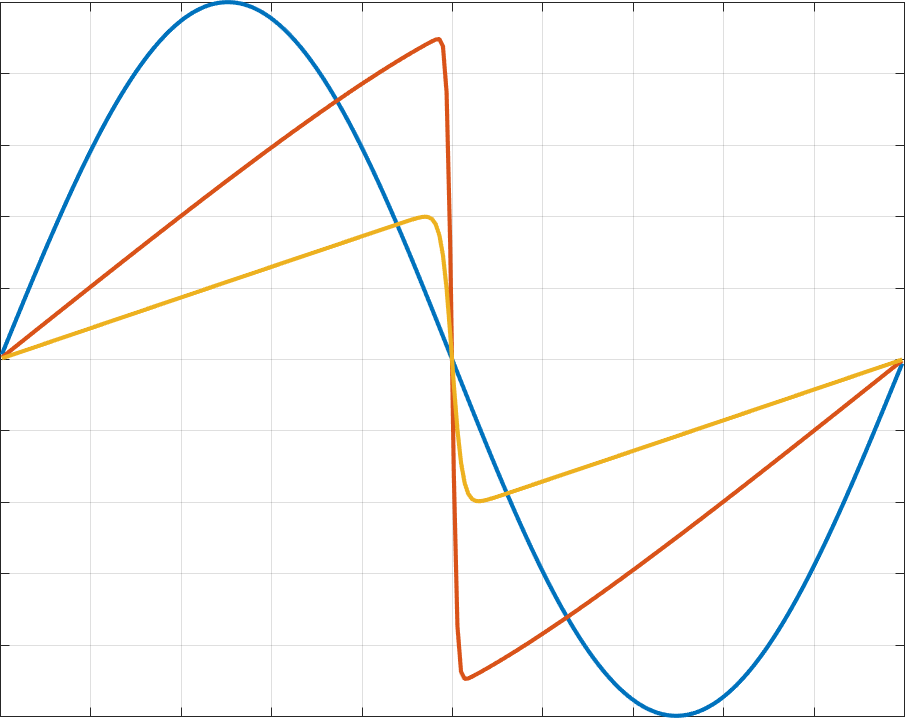
\includegraphics[width=.3\textwidth]{figs/burg_snaps.png}}
\hspace{.5em}
\subfloat[Modes (columns of $\bm{V}$)]{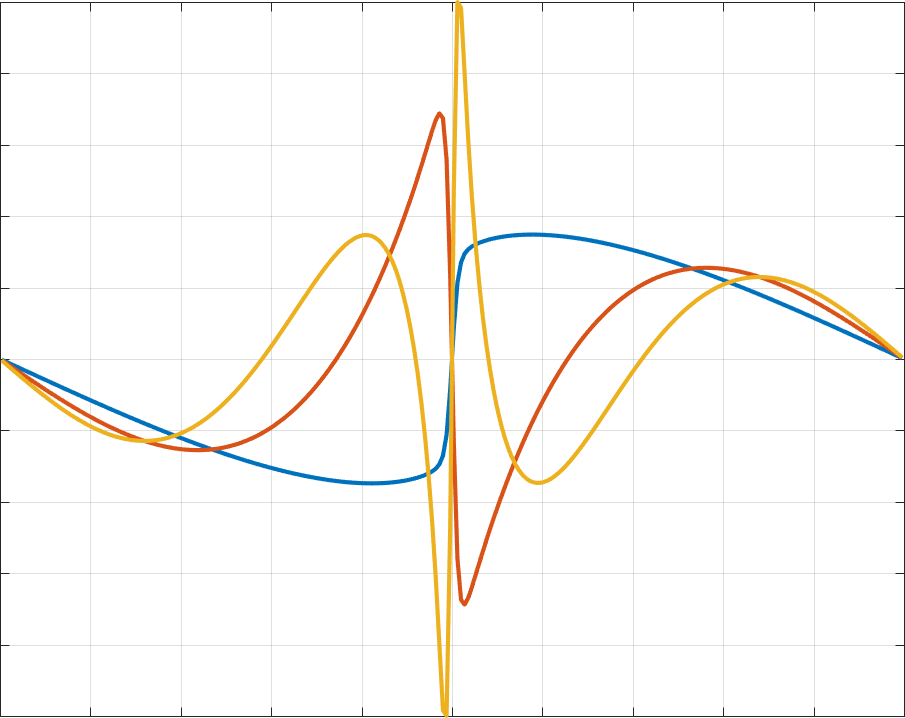
\includegraphics[width=.3\textwidth]{figs/burg3modes.png}}
\hspace{.5em}
\subfloat[Mode derivatives $\bm{Q}\bm{V}$]{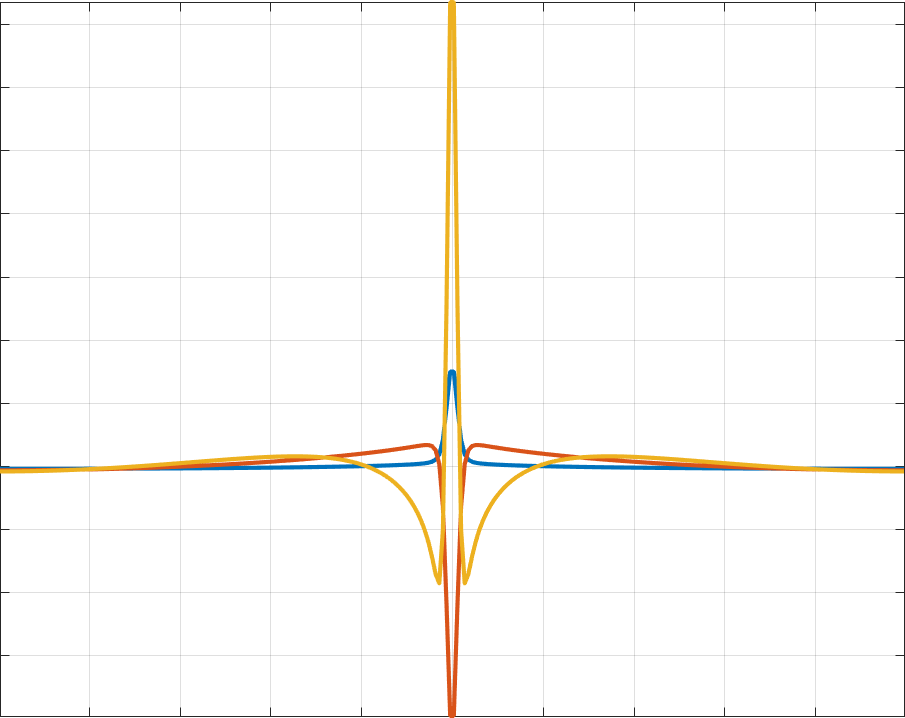
\includegraphics[width=.3\textwidth]{figs/burg3modes_diff.png}}
\caption{Solution snapshots, three POD modes, and mode derivatives for a shock solution of the viscous periodic Burgers' equation. }
\label{fig:modeQ}
\end{figure}

This example implies that the reduced basis matrix $\bm{V}$ can do a poor job of sampling the range of $\bm{Q}\bm{V}$, and that the test basis should contain additional vectors.  To remedy this issue, we borrow techniques from least squares Petrov-Galerkin ROMs \cite{carlberg2011efficient, carlberg2017galerkin} and enrich the test basis $\bm{V}_t$ with vectors spanning the range of $\bm{Q}\bm{V}$.  The test basis now spans a space which contains $\bm{1}, \bm{V}$, and $\bm{Q}\bm{V}$, and thus has a dimension of at most $2N+1$.  The dimension of $\bm{V}_t$ may also be smaller if the intersection of the range of the reduced basis matrix $\bm{V}$ and the range of $\bm{Q}\bm{V}$ and $\bm{1}$ is non-empty.  

We illustrate why this choice of test basis restores accuracy.  The entropy conservative flux for Burgers' equation corresponds to the discretization of the split form \cite{canuto2006spectral, chan2017discretely, maboudi2018conservative}
\[
\pd{u}{t} + \frac{1}{3}\LRp{\pd{u^2}{x}  + u\pd{u}{x}} = 0.
\]
An entropy conservative ROM without hyper-reduction is then given by 
\[
\bm{V}^T\bm{V}\td{u}{t} + \frac{1}{3}\bm{V}^T\LRp{\bm{Q}_t\bm{u}^2  + {\rm diag}\LRp{\bm{u}}\bm{Q}_t\bm{u}} = \bm{0}, \qquad \bm{u} = \bm{V}\bm{u}_N.
\]
It was shown in \cite{chan2017discretely, chenreview} that, for certain entropy conservative fluxes, the flux differencing procedure is equivalent in discretization of the split form.  Thus, to ensure accurate evalution of the spatial formulation, the reduced matrix $\bm{Q}_t$ should accurately approximate mixed derivatives of the form ${\rm diag}(\bm{f})\bm{Q}\bm{g}$.  We quantify the accuracy of $\bm{Q}_t$ in approximating such terms with the following theorem:
\begin{theorem}
Let $\bm{f},\bm{g}$ denote vectors, and let $\bm{u}_1, \bm{u}_2$ denote solutions of the following problems
\begin{align*}
\bm{V}^T\bm{V}\bm{u}_1 &= \bm{V}^T \diag{\bm{f}}\bm{Q}\bm{g}\\
\bm{V}^T\bm{V}\bm{u}_2 &= \bm{V}^T \diag{\bm{f}}\bm{Q}_t\bm{g}.
\end{align*}
Then, the error $\bm{e} = \bm{u}_1-\bm{u}_2$ satisfies
\[
\nor{\bm{V}\bm{e}} \leq \nor{\bm{Q}} \LRp{\nor{\bm{f}-\bm{V}\bm{P}\bm{f}} \nor{\bm{g}} + \nor{\bm{f}}\nor{\bm{g}-\bm{V}\bm{P}\bm{g}}}.
\]
\label{thm:acc}
\end{theorem}
\begin{proof}
Since $\bm{Q}_t = \bm{P}_t^T\LRp{\bm{V}_t^T\bm{Q}\bm{V}_t}\bm{P}_t$, we can derive the estimate by adding and subtracting $\bm{P}_t^T\bm{V}_t^T \diag{\bm{f}}\bm{Q}\bm{g}$.  Straightforward manipulations give the following
\begin{align*}
\bm{V}^T\diag{\bm{f}}\LRp{\bm{Q}\bm{g} - \bm{Q}_t\bm{g}} =  
\bm{V}^T\diag{\bm{f}} \LRp{\bm{Q}\LRp{\bm{I}-\bm{V}_t\bm{P}_t}\bm{g} + \LRp{\bm{I}-\bm{V}_t\bm{P}_t}^T\bm{Q}\bm{g}}
\end{align*}
 \note{Add proof}
 \end{proof}

Theorem~\ref{thm:acc} does not account for hyper-reduction.   

\subsection{Hyper-reduction algorithm and target space}
\label{sec:hyperreducalgo}

In this work, we utilize the greedy algorithm for computing empirical cubature points and weights from \cite{an2008optimizing, hernandez2017dimensional}, which is described in Algorithm~\ref{alg:hr}.  Let $\bm{V}_{\rm target}$ be some matrix whose columns span some target space of functions to be integrated.  The algorithm approximates $\bm{V}_{\rm target}^T\bm{1}$ by $\bm{V}_{\rm target}\LRp{\mathcal{I},:}^T\bm{w}$.  The index set is constructed in a greedy fashion by selecting the row index of $\bm{V}_{\rm target}$ which is most positively parallel to the residual, then computing the weight vector which minimizes the residual through a (non-negative) least squares solve.  

\begin{algorithm}
\caption{Compute hyper-reduction s.t.\ $\bm{V}_{\rm target}^T\bm{w}_{\rm target} \approx \bm{V}_{\rm target}\LRp{\mathcal{I},:}^T\bm{w}$.}
\begin{algorithmic}[1]
\STATE \textbf{Input}: $\bm{V}_{\rm target}, \bm{w}_{\rm target}, tol$.
\STATE \textbf{Output}: $\mathcal{I}$, $\bm{w}$.
\STATE Set $\bm{b} = \bm{V}_{\rm target}^T\bm{w}_{\rm target}$.
\STATE Initialize residual $\bm{r} = \bm{b}$, $\mathcal{I} = \emptyset$.
\WHILE {$\nor{\bm{r}}/\nor{\bm{b}} > tol$}
        \STATE Select new index $i$ such that
        \[
        i = \argmin_i \tilde{\bm{V}}_{i}\bm{r}/\nor{\bm{r}}, \qquad
        \tilde{\bm{V}}_i = \bm{V}_{\rm target}(i,:) / \nor{\bm{V}_{\rm target}(i,:)}, \quad i \not\in \mathcal{I}.
        \]
        \STATE Set $\mathcal{I} = \mathcal{I} \cup \LRc{i}$.  
        \STATE Compute $\bm{w}$ using linear least squares
        \[
        \bm{w} = \argmin_{\bm{c}} \nor{\bm{V}_{\rm target}\LRp{\mathcal{I},:}^T\bm{c} - \bm{b}}.
        \]
        \IF {$\min \bm{w} \leq 0$}
                \STATE Recompute $\bm{w}$ using non-negative least squares 
                \[
                \argmin_{\bm{c} \geq 0} \nor{\bm{V}_{\rm target}\LRp{\mathcal{I},:}^T\bm{c} - \bm{b}}
                \]             
        \ENDIF
        \STATE Recompute $\bm{r} = \bm{b} - \bm{V}_{\rm target}\LRp{\mathcal{I},:}^T\bm{w}$.
\ENDWHILE
\end{algorithmic}
\label{alg:hr}
\end{algorithm}

Algorithm~\ref{alg:hr} requires both $\bm{V}_{\rm target}$ and $\bm{w}_{\rm target}$ as inputs. For all numerical experiments, we set $\bm{w}_{\rm target} = \Delta x \bm{1}$ and set $\bm{V}_{\rm target}$ to be the span of products of POD functions $\bm{V}$, such that
\[
\mathcal{R}\LRp{\bm{V}_{\rm target}} = {\rm span}\LRc{\bm{V}(:,i) \circ \bm{V}(:,j), \quad i,j = 1,\ldots, N}.
\]
This choice of target space ensures that the mass matrix $\Delta x \bm{V}^T\bm{V}$ is accurately approximated.  In practice, since many of the pointwise vector products $\bm{V}(:,i) \circ \bm{V}(:,j)$ are linearly dependent, we replace $\bm{V}_{\rm target}$ by a dimensionally reduced matrix computed using, for example, another application of the SVD.  %a randomized SVD \cite{halko2011finding, rsvd}.  

\begin{remark}
We note that the target space is designed to accurately approximate the mass matrix $\Delta x \bm{V}^T\bm{V}$, but does not take the test basis $\bm{V}_{t}$ into account.  It is thus possible to construct a hyper-reduced quadrature which accurately integrates the mass matrix but violates Assumption~\ref{ass:quad}.  We have not encountered this situation in our experiments; however, one can ensure that Assumption~\ref{ass:quad} is satisfied by checking if $\bm{V}_t\LRp{\mathcal{I},:}$ is non-singular and selecting additional points based on $\bm{V}_t$ as necessary.  
\end{remark}

 
\subsection{An entropy conservative hyper-reduced model on periodic domains}

To summarize, an entropy conservative reduced order model on periodic domains can be constructed using the following ingredients and steps:
\begin{enumerate}
\item Compute a reduced basis matrix $\bm{V}$ from snapshots of both the conservative variables and the entropy variables.  
\item Construct ``test'' basis matrices $\bm{V}_t$ to produce a compressed ``modal'' differentiation matrix $\hat{\bm{Q}}_t = \bm{V}_t^T\bm{Q}\bm{V}_t$.
\item Compute a hyper-reduced quadrature using Algorithm~\ref{alg:hr}.  
\item Construct the hyper-reduced nodal differentiation matrix $\bm{Q}_t = \bm{P}_t^T\hat{\bm{Q}}_t\bm{P}_t$ using the projection matrix onto the test basis $\bm{P}_t$.
\end{enumerate}

%: \note{summarize restrictions and assumptions on hyper-reduction, POD, and test basis.}
\begin{theorem}
Suppose that the hyper-reduced quadrature satisfies Assumption~\ref{ass:quad}.  Then, the semi-discrete formulation 
\begin{gather}
\bm{M}_N\td{\bm{u}_N}{t} + 2\bm{V}\LRp{\mathcal{I},:}^T\LRp{\bm{Q}_t \circ \bm{F}}\bm{1} = \bm{0} \label{eq:hrrom}\\
\bm{M}_N = \bm{V}\LRp{\mathcal{I},:}^T\bm{W}\bm{V}\LRp{\mathcal{I},:}, \qquad \bm{P} = \bm{M}_N^{-1}\bm{V}\LRp{\mathcal{I},:}^T\bm{W},\nonumber\\ 
\bm{v}_N = \bm{P}\bm{v}\LRp{\bm{V}\LRp{\mathcal{I},:}\bm{u}_N}, \qquad \tilde{\bm{v}} = \bm{V}\LRp{\mathcal{I},:}\bm{v}_N, \nonumber\\
\tilde{\bm{u}} = \bm{u}\LRp{\tilde{\bm{v}}}, \qquad \bm{F}_{ij} = \bm{f}_S\LRp{\tilde{\bm{u}}_i,\tilde{\bm{u}}_j},\nonumber
\end{gather}
discretely conserves entropy 
\[
\Delta x \bm{1}^T\td{S\LRp{\bm{V}\bm{u}_N}}{t} = 0.  
\]
Additionally, if the reduced basis $\bm{V}$ exactly represents $\bm{1}$, solutions of (\ref{eq:hrrom}) conserve global averages of the conservative variables.
\label{thm:hrromes}
\end{theorem}
\begin{proof}
Since the hyper-reduction preserves the skew-symmetry and zero row sums of $\bm{Q}_t$, the proof is identical in structure to the proof of Theorem~\ref{thm:esrom}.  
\end{proof}

\begin{remark}
It is not strictly necessary to use the hyper-reduced mass matrix 
\[
\bm{M}_N = \bm{V}\LRp{\mathcal{I},:}^T\bm{W}\bm{V}\LRp{\mathcal{I},:}
\]
 to construct an entropy conservative ROM.  For example, we can use the exact mass matrix $\bm{M}_N = \Delta x \bm{V}^T\bm{V}$ rather than the hyper-reduced mass matrix.  If the projection matrix $\bm{P}$ is defined accordingly, the resulting ROM remains entropy conservative.  However, we observe significantly larger errors when using the exact mass matrix instead of the hyper-reduced mass matrix.  
\end{remark}


We note that the flux matrix $\bm{F}$ is not computed explicitly, but instead is usually formed on the fly.  The computation of $\bm{F}$ constitutes a significant portion of the computational cost, but can be reduced for the full order model by exploiting the sparsity of $\bm{Q}$.  However, since the hyper-reduced matrix $\bm{Q}_t$ is fully dense, the ROM (\ref{eq:hrrom}) requires $O(N_s^2)$ nonlinear flux evaluations, in contrast to the typical $O(N_s)$ nonlinear function evaluations required for a typical hyper-reduced model.  


\subsection{Hyper-reduction and entropy dissipation}
\label{sec:diss}
Given an entropy conservative ROM with hyper-reduction, we can construct an entropy stable ROM by adding appropriate entropy-dissipative viscosity terms.  Recall that the artificial diffusion matrix $\bm{K}$ in (\ref{eq:esvisc}) does not depend nonlinearly on $\bm{u}$.  Thus, typical model reduction techniques compress such operators using Galerkin projection, e.g., $\bm{V}^T\bm{K}\bm{V}$.  However, since one cannot in general show that this operator dicretely dissipates entropy, we discuss two treatments of the viscous terms which are provably entropy dissipative.  

This section introduces hyper-reduction procedures for $\bm{K}$ which provide a provable discrete dissipation of entropy.  We seek to mimic the entropy balance of the full order model in (\ref{eq:entropybalancefom}).  Suppose the reduced order model is given by 
\[
\bm{M}_N\td{\bm{u}_N}{t} + 2\bm{V}\LRp{\mathcal{I},:}^T\LRp{\bm{Q}_t \circ \bm{F}}\bm{1} + \bm{d}(\bm{u}_N)= \bm{0}
\]
where $\bm{d}(\bm{u})$ is some hyper-reduced approximation to the viscous terms.  Theorem~\ref{thm:hrromes} gives that the entropy balance of the reduced order model is
\[
\Delta x \bm{1}^T\td{S\LRp{\bm{V}\bm{u}_N}}{t} = -\bm{v}_N^T\bm{d}(\bm{u}_N).
\]
We will design hyper-reduced treatments of the viscous terms such that $\bm{v}_N^T\bm{d}(\bm{u}_N) \geq 0$, which implies that the reduced model is entropy stable.  

Let $\bm{D}$ denote the $(K-1)\times K$ difference matrix
\[
\bm{D} = \frac{1}{\Delta x}\begin{bmatrix}
1 & -1 &&& \\
 & 1 & -1 && \\
 & & \ddots & \ddots&\\
&  & & 1 & -1
\end{bmatrix}.
\]
The artificial diffusion matrix in (\ref{eq:esvisc}) can be decomposed as $\bm{K} = \bm{D}^T\bm{D}$.  To construct hyper-reduced diffusion terms, we first compute (using the SVD) an auxiliary basis $\bm{V}_{\bm{D}}$ for $\bm{D}\bm{V}$, where $\bm{V}$ is the reduced basis matrix.  We then perform hyper-reduction to compute weights and sampled row indices such that 
\[
\bm{V}_{\bm{D}}^T\bm{V}_{\bm{D}} \approx \bm{V}_{\bm{D}}\LRp{\mathcal{I}_{\bm{D}},:}^T \bm{W}_{\bm{D}}\bm{V}_{\bm{D}}\LRp{\mathcal{I}_{\bm{D}},:}.
\]

We can now construct entropy-dissipative diffusion terms using this second hyper-reduction of $\bm{D}$.  The first treatment is relatively straightforward, and simply samples rows of $\bm{D}$ corresponding to indices $\mathcal{I}_{\bm{D}}$.  The viscous terms $\bm{K}\bm{u}$ in the full order model are approximated using the sparse hyper-reduced matrix $\bm{D}\LRp{\mathcal{I}_{\bm{D}},:}$
\begin{equation}
%\bm{K}\bm{u} \approx 
\bm{d}(\bm{u}_N) = \bm{D}\LRp{\mathcal{I}_{\bm{D}},:}^T \bm{W}_{\bm{D}} \bm{D}\LRp{\mathcal{I}_{\bm{D}},:}\tilde{\bm{u}}.
\label{eq:visc1}
\end{equation}
Since the entropy-projected conservative variables $\tilde{\bm{u}}$ are mappings of the projected entropy variables $\bm{V}\bm{v}_N$, repeating the steps used to derive (\ref{eq:entropydissfom}) yields that the entropy dissipation of (\ref{eq:visc1}) is 
\begin{align*}
\bm{v}_N^T\bm{V}^T\bm{D}^T\LRp{\mathcal{I}_{\bm{D}},:}^T \bm{W}_{\bm{D}} \bm{D}\LRp{\mathcal{I},:}\tilde{\bm{u}} &= 
\tilde{\bm{v}}^T\bm{D}^T\LRp{\mathcal{I}_{\bm{D}},:}^T \bm{W}_{\bm{D}} \bm{D}\LRp{\mathcal{I},:}\bm{u}\LRp{\tilde{\bm{v}}}
\\
&= \sum_{i\in \mathcal{I}_{\bm{D}}} \frac{w_{\bm{D},i}}{\Delta x^2} \LRl{\pd{\bm{u}}{\bm{v}}}_{i,i+1} \LRp{\tilde{\bm{v}}_i - \tilde{\bm{v}}_{i+1}}^2.
\end{align*}

The second treatment of the diffusion terms is motivated by approaches taken in \cite{carpenter2014entropy, chen2017entropy, zakerzadeh2017entropy, upperman2019entropy}.  Recall that, using the mean value theorem, the $i$th entry of $\bm{D}\bm{u}$ is
\begin{equation}
\LRp{\bm{D}\bm{u}}_i = \bm{u}_i - \bm{u}_{i+1} = \LRl{\pd{\bm{u}}{\bm{v}}}_{i,i+1} \LRp{\bm{v}(\bm{u}_i)-\bm{v}(\bm{u}_{i+1})} = \LRl{\pd{\bm{u}}{\bm{v}}}_{i,i+1}  \LRp{\bm{D}\bm{v}(\bm{u})}_i,
\label{eq:meanval}
\end{equation}
where $\LRl{\pd{\bm{u}}{\bm{v}}}_{i,i+1}$ is $\pd{\bm{u}}{\bm{v}}$ evaluated at some intermediate state between $\bm{u}_i$ and $\bm{u}_{i+1}$.  This motivates a hyper-reduction based on sampling and weighting rows of $\bm{D}$ applied to the vector of entropy variables $\bm{v}(\bm{u})$.  The diffusion terms can be approximated by 
\begin{equation}
%\bm{K}\bm{u} \approx 
\bm{d}(\bm{u}_N) = \bm{V}^T\bm{D}\LRp{\mathcal{I}_{\bm{D}},:}^T \bm{W}_{\bm{D}} \bm{H} \bm{D}\LRp{\mathcal{I}_{\bm{D}},:}\bm{V} \bm{v}_N
\label{eq:visc2}
\end{equation}
where $\bm{v}_N$ are coefficients of the projected entropy variables in (\ref{eq:hrrom}), $\bm{W}_{\bm{D}}$ is a diagonal matrix of positive weights $w_{\bm{D},i}$, and $\bm{H}$ is a diagonal matrix containing entries of the Jacobian $\pd{\bm{u}}{\bm{v}}$\footnote{Recall that matrices are treated as Kronecker products, and that the diagonal entries of $\bm{H}_{ii}$ correspond to block matrices acting on the vector of solution components at a point.} evaluated at all hyper-reduced points in $\mathcal{I}_{\bm{D}}$ 
\[
\bm{H}_{ii} = \LRl{\pd{\bm{u}}{\bm{v}}}_{\bm{u} = \bar{\bm{u}}_i}, \qquad \bar{\bm{u}}_i = \frac{\tilde{\bm{u}}_i + \tilde{\bm{u}}_{i+1}}{2}.
\]
Since we do not know the intermediate state used to evaluate $\LRl{\pd{\bm{u}}{\bm{v}}}_{i,i+1}$ in (\ref{eq:meanval}), 
we have arbitrarily chosen to evaluate $\pd{\bm{u}}{\bm{v}}$ at the average of the entropy-projected conservative values $\tilde{\bm{u}}_i$ and $\tilde{\bm{u}}_{i+1}$.  Since the diagonal entries of $\bm{W}_{\bm{D}}$ are positive and $\pd{\bm{u}}{\bm{v}}$ is symmetric positive definite (for physically relevant values of $\tilde{\bm{u}}$), the entropy dissipation of the hyper-reduced diffusion term is given by
\[
\bm{v}_N^T\bm{V}^T\bm{D}^T\LRp{\mathcal{I}_{\bm{D}},:}^T \bm{W}_{\bm{D}} \bm{H} \bm{D}\LRp{\mathcal{I},:}\bm{V} \bm{v}_N = 
\sum_{i\in \mathcal{I}_{\bm{D}}} \frac{w_{\bm{D},i}}{\Delta x^2} \LRl{\pd{\bm{u}}{\bm{v}}}_{\bm{u}=\bar{\bm{u}}_i} \LRp{\tilde{\bm{v}}_i - \tilde{\bm{v}}_{i+1}}^2.
\]
This implies that the dissipation of entropy produced by the hyper-reduced approximation of the viscous terms (\ref{eq:visc2}) also mimics the dissipation of entropy (\ref{eq:entropydissfom}) derived for the full order model.
The difference between the hyper-reduction treatments of viscosity (\ref{eq:visc1}) and (\ref{eq:visc2}) are that (\ref{eq:visc1}) relies explicitly on the fact that $\bm{D}$ is a two-point finite volume difference matrix, which enables the use of the mean value theorem in deriving a statement of entropy dissipation.   The first approach (\ref{eq:visc1}) results in a simpler online phase, though it involves larger matrices compared to the second approach.  The second approach (\ref{eq:visc2}) is not limited to finite volume methods, and is entropy dissipative for any choice of differentiation matrix $\bm{D}$.  Both approaches require computing an additional set of hyper-reduced points during the offline phase.  

\begin{remark}
The hyper-reduction treatments of viscosity described in this section can also be applied to interface dissipation, such as local Lax-Friedrichs penalization.  %However, these dissipation terms depend on the resolution of the full order model.  
\end{remark}

We note that, in practice, a naive approximation of diffusive terms $\bm{K}\bm{u}$ by
\begin{equation}
%\bm{K}\bm{u} \approx 
\bm{d}(\bm{u}_N) = \bm{V}^T\bm{K}\bm{V}\bm{P}\tilde{\bm{u}},
\label{eq:visc3}
\end{equation}
is often effective.  This approach is simpler to implement than (\ref{eq:visc1}),(\ref{eq:visc2}), and does not require a second set of hyper-reduced points.  We are unable to show that this treatment is provably entropy dissipative.  However, in all experiments, we observe that $\bm{v}_N^T\bm{V}^T\bm{K}\bm{V}\bm{P}\tilde{\bm{u}} \geq 0$, which implies that entropy is discretely dissipated.  

\section{Weak imposition of boundary conditions}
\label{sec:6}
Until now, we have assumed periodic domains.  In this section, we discuss how to extend the construction of entropy stable ROMs to the non-periodic case.  Boundary conditions are weakly imposed through a numerical flux and a ``hybridized'' summation by parts operator \cite{chan2017discretely}.  

In the non-periodic case, the matrix $\bm{Q}$ is nearly skew-symmetric, such that it satisfies a summation by parts property
\begin{equation}
\bm{Q} = \frac{1}{2}\begin{bmatrix}
-1 & 1 & & \\
-1 & 0 & \ddots &\\
 &\ddots &\ddots &1\\
  & & -1 &1\\
\end{bmatrix}, \qquad \bm{Q} + \bm{Q}^T = \bm{B}_{\rm SBP} = 
\begin{bmatrix}
-1& && \\
&0 &&\\
& &\ddots &\\
& &&1\\
\end{bmatrix}
\label{eq:fomsbp}
\end{equation}
A non-periodic full order model can be expressed as 
\begin{align}
\Delta x \td{\bm{u}_h}{t} + 2\LRp{{\bm{Q}}\circ \bm{F}}\bm{1} + \bm{B}_{\rm SBP}\LRp{\bm{f}^* - \bm{f}(\bm{u})} = \bm{0},
\label{eq:esbc}
\end{align}
where $\bm{f}^* = \LRs{\bm{f}^*_0, 0,\ldots, 0, \bm{f}^*_K}^T$ is a vector containing values of the nonlinear flux at the boundary points.  
Following \cite{chen2017entropy}, a boundary numerical flux $\bm{f}^*$ is entropy stable if 
\begin{equation}
\psi\LRp{\bm{u}} - \bm{v}(\bm{u})^T\bm{f}^* \leq \bm{0}.%, \qquad \text{check this!}}
\label{eq:esbflux}
\end{equation}
The flux is referred to as entropy conservative if the inequality is an equality.  If an entropy stable or entropy conservative flux $\bm{f}_S(\bm{u}_L,\bm{u}_R)$ is used to evaluate both the volume and surface flux, then the resulting full order model given by (\ref{eq:esbc}) is also entropy stable or entropy conservative \cite{tadmor1987numerical, parsani2015entropy, chen2017entropy}.  

Extending entropy conservative treatments of boundary conditions to the reduced order model is less straightforward due to fact that reduced matrices do not satisfy the same SBP property (\ref{eq:fomsbp}).  If the full order matrix $\bm{Q}$ satisfies the SBP property, then the hyper-reduction of $\bm{Q}$ satisfies a \textit{generalized} SBP property \cite{fernandez2014generalized} 
\[
\bm{Q}_t + \bm{Q}_t^T = \bm{E}^T\bm{B}\bm{E}, \qquad \bm{Q}_t = \bm{P}_t^T\bm{V}_t^T\bm{Q}\bm{V}_t\bm{P}_t.
\]
where the matrices $\bm{B}$ and $\bm{E}$ encode scaling by normals and evaluation at boundary points.  In 1D, these matrices are given by
\[
\bm{B} = \begin{bmatrix}-1 & \\ & 1\end{bmatrix}, \qquad \bm{E} = \bm{V}_{bt}\bm{P}_t, \qquad \bm{V}_{bt} = \begin{bmatrix}\bm{V}_t(1,:) \\ \bm{V}_t(N,:)\end{bmatrix}.
\]
where $\bm{V}_t(:,1), \bm{V}_t(:,K)$ denote the first and last columns (corresponding to points on the boundary) of the test basis matrix $\bm{V}_t$.  

For linear problems, it is possible to impose energy stable boundary conditions by combining generalized SBP operators with appropriate simultaneous approximation terms (SATs) \cite{fernandez2014review, fernandez2018simultaneous}.  However, due to the presence of $\bm{E}$ within the boundary term $\bm{E}^T\bm{B}\bm{E}$, the accurate and entropy stable imposition of nonlinear boundary conditions using generalized SBP SATs remains an open problem \cite{crean2018entropy, chan2018efficient, chenreview}. We address this issue by constructing a \textit{hybridized} SBP operator (also referred to as a decoupled SBP operator) \cite{chan2017discretely, chan2019skew}
\[
\bm{Q}_{h} = \frac{1}{2}\begin{bmatrix}
\bm{Q}_t - \bm{Q}_t^T & \bm{E}^T\bm{B} \\
-\bm{B}\bm{E} & \bm{B}
\end{bmatrix}.
\]
Note that $\bm{Q}_h$ satisfies a block version of the standard summation by parts property by construction
\[
\bm{Q}_h + \bm{Q}_h^T = \bm{B}_h = \begin{bmatrix}
\bm{0} & \\
& \bm{B} \end{bmatrix},  
\]
where $\bm{B}_h$ is diagonal and does not involve the boundary evaluation matrix $\bm{E}$.  

A more subtle property is that $\bm{Q}_h\bm{1} = \bm{0}$ \cite{chan2019skew}.  Note that the full order matrix $\bm{Q}$ in (\ref{eq:fomsbp}) satisfies $\bm{Q}\bm{1} = \bm{0}$.  Then, since $\bm{1}$ is exactly representable in the test basis $\bm{V}_t$, $\bm{V}_t\bm{P}_t\bm{1} = \bm{1}$, and
\[
\bm{Q}_t = \bm{P}_t^T\bm{V}_t^T\bm{Q}\bm{V}_t\bm{P}_t\bm{1} = \bm{P}_t^T\bm{V}_t^T\bm{Q}\bm{1} = \bm{0}.
\]
This implies that $\bm{Q}_h\bm{1}$ simplifies to
\[
\bm{Q}_h \bm{1} =  \frac{1}{2}\begin{bmatrix}
\bm{Q}_t \bm{1} - \bm{Q}_t^T \bm{1} + \bm{E}^T\bm{B} \bm{1} \\
- \bm{B}\bm{E} \bm{1} + \bm{B}
\end{bmatrix}=\frac{1}{2}\begin{bmatrix}
- \bm{Q}_t^T \bm{1} + \bm{E}^T\bm{B} \bm{1} \\
\bm{0}
\end{bmatrix},
\]
where we have used that $\bm{Q}_t\bm{1} = \bm{0}$ and that (\ref{eq:preproduce}) implies $\bm{E}\bm{1} = \bm{1}$.   Here, we abuse notation by letting $\bm{1}$ denote any arbitrary length vector of all ones.  Furthermore, since $\bm{Q}_t$ satisfies a generalized SBP property,
\[
- \bm{Q}_t^T \bm{1} + \bm{E}^T\bm{B} \bm{1} = \LRp{-\bm{Q}_t^T + \bm{E}^T\bm{B}\bm{E}} \bm{1} = \bm{Q}_t \bm{1} = \bm{0}.
\]
we conclude that $\bm{Q}_h\bm{1} = \bm{0}$.

By replacing $\bm{Q}_t$ in (\ref{eq:hrrom}) with $\bm{Q}_h$, we can impose boundary conditions weakly through a numerical flux $\bm{f}^*$.  We define $\bm{V}_b$ as the matrix which evaluates the reduced basis at boundary points $\LRc{-1,1}$, and define $\bm{V}_h$ as the matrix which evaluates the reduced basis at both boundary points and hyper-reduced volume points
\[
\bm{V}_{b} = \begin{bmatrix}\bm{V}(1,:) \\ \bm{V}(N,:)\end{bmatrix}, \qquad \bm{V}_h = \begin{bmatrix}
\bm{V}\LRp{\mathcal{I},:}\\
\bm{V}_{b}
\end{bmatrix}.
\]
We then have the following theorem:
\begin{theorem}
If the boundary flux $\bm{f}^*$ is entropy stable in the sense of (\ref{eq:esbflux}), then the following hyper-reduced ROM 
\begin{gather}
\bm{M}_N\td{\bm{u}_N}{t} + 2\bm{V}_h^T\LRp{\bm{Q}_h \circ \bm{F}}\bm{1} + \bm{V}_{b}^T\bm{B}\LRp{\bm{f}^* - \bm{f}(\tilde{\bm{u}}_b)} = \bm{0} \label{eq:esbchr}\\
\bm{v}_N = \bm{P}\bm{v}\LRp{\bm{V}\LRp{\mathcal{I},:}\bm{u}_N}, \qquad \tilde{\bm{v}} = 
\bm{V}_h
\bm{v}_N, \qquad \tilde{\bm{v}}_b = \bm{V}_b\bm{v}_N, \nonumber\\
\tilde{\bm{u}} = \bm{u}\LRp{\tilde{\bm{v}}}, \qquad \bm{F}_{ij} = \bm{f}_S\LRp{\tilde{\bm{u}}_i,\tilde{\bm{u}}_j}, \qquad  \tilde{\bm{u}}_b = \bm{u}\LRp{\tilde{\bm{v}}_b}\nonumber
\end{gather}
is also entropy stable such that
\[
\td{S\LRp{\bm{V}\bm{u}_N}}{t} \leq 0,
\]
with equality holding for an entropy conservative flux.
\label{thm:esbchr}
\end{theorem}
\begin{proof}
The proof is identical in structure to the proof of Theorem 1 in \cite{chan2017discretely}.  We reproduce it here for completeness.
Testing with $\bm{v}_N$ and using the summation by parts property of $\bm{Q}_h$ then yields 
\begin{align*}
\td{S\LRp{\bm{V}\bm{u}_N}}{t}  + \tilde{\bm{v}}^T\LRp{\LRp{\bm{Q}_h-\bm{Q}_h} \circ \bm{F}}\bm{1} + \tilde{\bm{v}}_b^T\bm{B}\bm{f}^*  = \bm{0}.
\end{align*}
Here, we have used that, by the consistency of the entropy conservative flux (\ref{eq:esflux}), the diagonal entries of $\bm{F}$ are $\bm{F}_{ii} = \bm{f}\LRp{\tilde{\bm{u}}_i}$.  Thus, since $\bm{B}_h$ is also diagonal,
\[
\LRp{\bm{B}_h\circ\bm{F}}\bm{1} = \bm{B} \bm{f}(\tilde{\bm{u}}_b).
\]
Expanding out the term $\tilde{\bm{v}}^T\LRp{\LRp{\bm{Q}_h-\bm{Q}_h^T} \circ \bm{F}}\bm{1}$ and using skew-symmetry of $\bm{Q}_h-\bm{Q}_h^T$ yields
\begin{align*}
\tilde{\bm{v}}^T\big(\underbrace{\LRp{\bm{Q}_h-\bm{Q}_h^T}}_{\bm{S}_h} \circ \bm{F}\big)\bm{1} &= 
%\sum_{ij} \LRp{\bm{S}_h}_{ij} \tilde{\bm{v}}_i^T\bm{f}_S\LRp{\tilde{\bm{u}}_i,\tilde{\bm{u}}_j} \\
%&= 
\frac{1}{2}\sum_{ij} \LRp{\bm{S}_h}_{ij} \LRp{\tilde{\bm{v}}_i-\tilde{\bm{v}}_j}^T\bm{f}_S\LRp{\tilde{\bm{u}}_i,\tilde{\bm{u}}_j}\\
&= \frac{1}{2}\sum_{ij} \LRp{\bm{Q}_h-\bm{Q}_h^T}_{ij} \LRp{\psi(\tilde{\bm{u}}_i)-\psi(\tilde{\bm{u}}_j)}\\
&= \sum_{ij} \LRp{\bm{Q}_h}_{ij} \LRp{\psi(\tilde{\bm{u}}_i)-\psi(\tilde{\bm{u}}_j)} = {\psi(\tilde{\bm{u}})^T\bm{Q}_h\bm{1} - \bm{1}^T\bm{Q}_h\psi(\tilde{\bm{u}})}\\
& = -\bm{1}^T\bm{B}_h\psi(\tilde{\bm{u}}) = -\bm{1}^T\bm{B}\psi(\tilde{\bm{u}}_b),
\end{align*}
where we have used that $\bm{Q}_h\bm{1} = \bm{0}$ and the SBP property in the last two lines.  Using that $\bm{B}$ is diagonal, straightforward manipulations imply that
\[
\td{S\LRp{\bm{V}\bm{u}_N}}{t}  - \bm{1}^T\bm{B}\LRp{\psi(\tilde{\bm{u}}_b)-\tilde{\bm{v}}_b^T\bm{f}^*}  = \bm{0}.
\]
If the flux is entropy stable, then $\td{S\LRp{\bm{V}\bm{u}_N}}{t} \leq 0$, with equality holding if the flux is entropy conservative.
\end{proof}

%\note{Discuss issues with high order accuracy and entropy stability for SBP \cite{chan2018efficient}.}

\section{Extension to higher dimensions}
\label{sec:7}

\subsection{Periodic domains}
For periodic domains, the extension to higher spatial dimensions is relatively straightforward.  We provide a concrete construction of matrices and formulations in two dimensions.  For finite volume methods on a $K \times K$ structured quadrilateral elements of size $\Delta x \times \Delta x$, differentiation matrices along each coordinate direction can be constructed as Kronecker products of one-dimensional matrices.  Let $\bm{Q}_{\rm 1D}$ denote the one-dimensional periodic differentiation matrix defined in (\ref{eq:Qmat}).  The differentiation matrix along the $i$th coordinate direction $\bm{Q}^i$ can be constructed as follows
\[
\bm{Q}^1 = \bm{Q}_{\rm 1D}\otimes \Delta x \bm{I}, \qquad \bm{Q}^2 = \Delta x\bm{I} \otimes \bm{Q}_{\rm 1D}.
\]
Given a basis matrix $\bm{V}$ and indices of hyper-reduced points $\mathcal{I}$, we can introduce test basis matrices $\bm{V}^i_t$ such that the range of  $\bm{V}^i_t$ is equal to the direct sum of the ranges of $\bm{V}$ and $\bm{Q}^i\bm{V}$
\[
\mathcal{R}\LRp{\bm{V}^i_t} = \mathcal{R}\LRp{\begin{bmatrix}\bm{V} &\bm{Q}^i\bm{V}\end{bmatrix}}, \qquad i = 1,\ldots,d.
%\mathcal{R}\LRp{\bm{V}^y_t} = \mathcal{R}\LRp{\begin{bmatrix}\bm{V} &\bm{Q}^y\bm{V}\end{bmatrix}}.
\]
Note that, unlike the 1D case, the test bases differ along each coordinate direction.  However, the dimension of the range of each test basis $\bm{V}_t^i$ is still at most $2N+1$.  
We can now define hyper-reduced projection matrices
\begin{align*}
\bm{P}^i_t = \LRp{\bm{V}^i_t\LRp{\mathcal{I},:}^T\bm{W}\bm{V}^i_t\LRp{\mathcal{I},:}}^{-1}\bm{V}^i_t\LRp{\mathcal{I},:}^T\bm{W}.%,\\
%\bm{P}^y_t = \LRp{\bm{V}^y_t\LRp{\mathcal{I},:}^T\bm{W}\bm{V}^y_t\LRp{\mathcal{I},:}}^{-1}\bm{V}^y_t\LRp{\mathcal{I},:}^T\bm{W}.
\end{align*}
These test bases can be used to construct reduced matrices $\bm{Q}_t^i$ %, \bm{Q}_t^y$ 
\[
\bm{Q}_t^i = \LRp{\bm{P}^i_t}^T\LRp{\LRp{\bm{V}^i_t}^T\bm{Q}^i\bm{V}^i_t}\bm{P}^i_t,
% \qquad 
%\bm{Q}_t^y = \LRp{\bm{P}^y_t}^T\LRp{\LRp{\bm{V}^y_t}^T\bm{Q}^y\bm{V}^y_t}\bm{P}^y_t.
\]
which are used to construct an entropy stable reduced order model in $d$ dimensions
\begin{gather}
\bm{M}_N\td{\bm{u}_N}{t} + \sum_{i=1}^d 2\bm{V}\LRp{\mathcal{I},:}^T\LRp{\bm{Q}^i_t \circ \bm{F}^i}\bm{1} = \bm{0} \label{eq:hrromd}\\
\bm{M}_N = \Delta x^2 \bm{V}^T\bm{V}, \qquad \bm{F}^i_{jk} = \bm{f}^i_S\LRp{\tilde{\bm{u}}_j,\tilde{\bm{u}}_k}.\nonumber
%\bm{M}_N = \bm{V}\LRp{\mathcal{I},:}^T\bm{W}\bm{V}\LRp{\mathcal{I},:}, \qquad \bm{P} = \bm{M}_N^{-1}\bm{V}\LRp{\mathcal{I},:}^T\bm{W},\nonumber\\ 
%\bm{v}_N = \bm{P}\bm{v}\LRp{\bm{V}\LRp{\mathcal{I},:}\bm{u}_N}, \qquad \tilde{\bm{v}} = \bm{V}\LRp{\mathcal{I},:}\bm{v}_N, \nonumber\\
%\tilde{\bm{u}} = \bm{u}\LRp{\tilde{\bm{v}}}, \qquad ,\nonumber
\end{gather}
Here, $\bm{f}^i_S\LRp{\bm{u}_L,\bm{u}_R}$ is the entropy conservative flux in the $i$th coordinate direction and $\bm{M}_N$ is the mass matrix as defined in (\ref{eq:hrrom}).  We can show that (\ref{eq:hrromd}) is entropy conservative by repeating steps in the proof of Theorem~\ref{thm:hrromes} for each coordinate direction.  

\subsection{Non-periodic domains}

Non-periodic domains and boundary conditions can be treated by combining hybridized SBP operators and a weak imposition of boundary conditions as was done in the 1D hyper-reduced formulation (\ref{eq:esbchr}).  Without loss of generality, we assume a square domain with $4$ boundary faces, each of which is discretized by $K$ intervals of size $\Delta x$.  We assume we are given values of the outward normal vector $\bm{n}$ on the domain boundary
\[
\bm{n} = \LRs{n_1, \ldots, n_d}^T.
\]
We can enforce non-periodic boundary conditions through introducing numerical fluxes at boundary points.  However, the number of boundary points scales with $K$, the number of elements in the full order model along one coordinate direction.  To ensure that the cost of the reduced order model scales with the number of modes $N$ rather than the dimension of the full order model, we must apply an additional hyper-reduction to approximate boundary terms by a weighted combination of sub-sampled boundary points.  

Let $\bm{V}_b$ denote the matrix whose columns correspond to values of the reduced basis at boundary points.  Let $\mathcal{I}_b$ denote a sub-sampled set of $N_b$ boundary points, and let $g$ denote a nonlinear function.  We then approximate the boundary inner product 
\[
\bm{V}_b^Tg(\bm{V}_b\bm{u}_N) \approx \bm{V}_b\LRp{\mathcal{I}_b,:}^T \bm{W}_b g\LRp{\bm{V}_b\LRp{\mathcal{I}_b,:}}.
\]
where $\bm{W}_b$ is a diagonal matrix whose entries consist of positive weights
\[
\bm{W}_b = {\rm diag}\LRp{\bm{w}_b}.
\]
We can now define the $N_b\times N_b$ operators $\bm{B}^1, \bm{B}^2$ as the diagonal matrices whose entries consist of weighted component values of outward normals on the boundary 
\[
\bm{B}^i = {\rm diag}\LRp{\bm{n}^i} \bm{W}_b,
\]
where $\bm{n}^i$ is a vector containing the values of the component $n_i$ at boundary points.  

We can now construct hybridized SBP operators under both volume and boundary hyper-reduction.  Let $\bm{V}_{bt}$ be the matrix which evaluates the $i$th test basis at face points.  Then, we can define $\bm{E}_i$ as the matrix which extrapolates from hyper-reduced volume points to boundary points through projection onto the $i$th test basis
\[
\bm{E}_i = \bm{V}_{bt}^i\LRp{\mathcal{I}_b,:}\bm{P}^i_t.  
\]
The hybridized SBP operator for differentiation along the $i$th coordinate is then
\[
\bm{Q}_h^i = \begin{bmatrix}
\bm{Q}^i_t - \LRp{\bm{Q}^i_t}^T & \bm{E}_i^T\bm{B}^i \\ 
-\bm{B}^i\bm{E}_i & \bm{B}^i
\end{bmatrix}.
\]

These operators can be used to construct a hyper-reduced formulation in higher dimensions
\begin{gather}
\bm{M}_N\td{\bm{u}_N}{t} + \sum_{i=1}^d \LRp{2\bm{V}\LRp{\mathcal{I},:}^T\LRp{\bm{Q}^i_h \circ \bm{F}^i}\bm{1} + \bm{V}_b\LRp{\mathcal{I}_b,:}^T\bm{B}^i\LRp{\bm{f}_i^* - \bm{f}_i(\bm{u}_b)}} = \bm{0} \label{eq:hrromdbc},%\\
\end{gather}
where $\bm{M}_N$ and $\bm{F}^i$ are as defined in (\ref{eq:hrromd}), and $\bm{f}_i(\bm{u}), \bm{f}_i^*$ are the $i$th components of the flux function and boundary numerical flux, respectively.  

In contrast to the 1D case, additional steps are necessary to ensure that entropy stability is preserved under this boundary hyper-reduction.  Recall that the proof of entropy stability for 1D non-periodic domains in Theorem~\ref{thm:esbchr} requires that $\bm{Q}_h\bm{1} = \bm{0}$.  The analogous proof of entropy stability in multiple dimensions requires that $\bm{Q}^i_h\bm{1} = \bm{0}$ for $i = 1,\ldots, d$.  However, this is not automatically satisfied.  Expanding out $\bm{Q}^i_h\bm{1}$ yields
\[
\bm{Q}^i_h\bm{1} = \begin{bmatrix}
\bm{Q}^i_t\bm{1} - \LRp{\bm{Q}^i_t}^T\bm{1} + \bm{E}_i^T\bm{B}^i \bm{1}\\
\bm{0}
\end{bmatrix}= \begin{bmatrix}
-\LRp{\bm{Q}^i_t}^T\bm{1} + \bm{E}_i^T\bm{B}^i \bm{1}\\
\bm{0}
\end{bmatrix}.
\]
In general, $-\LRp{\bm{Q}^i_t}^T\bm{1} + \bm{E}^T\bm{B}^i \bm{1}\neq 0$, so $\bm{Q}^i_h\bm{1} \neq \bm{0}$ and the proof of entropy stability does not hold.  To enforce that $\bm{Q}^i_h\bm{1} = \bm{0}$, we impose constraints on the boundary weights $\bm{w}_b$.  Note that 
\begin{align*}
-\LRp{\bm{Q}^i_t}^T\bm{1} + \bm{E}^T\bm{B}^i \bm{1} &= -\LRp{\bm{P}^i_t}^T\bm{V}_t^T\bm{Q}\bm{V}_t\bm{P}^i_t\bm{1} + \LRp{\bm{P}^i_t}^T\LRp{\bm{V}^i_{bt}\LRp{\mathcal{I}_b,:}}^T\bm{B}^i\bm{1}\\
&= \LRp{\bm{P}^i_t}^T\LRp{-\LRp{\bm{V}^i_t}^T\bm{Q}\bm{1} + \LRp{\bm{V}^i_{bt}}\LRp{\mathcal{I}_b,:}^T{\rm diag}\LRp{\bm{n}^i}\bm{w}_b}.
\end{align*}
where we have used that $\bm{V}^i_t\bm{P}^i_t\bm{1} = \bm{1}$.  Thus, to ensure that $\bm{Q}^i_h\bm{1} = 0$, it is sufficient to guarantee that
\begin{equation}
\LRp{\bm{V}^i_{bt}}\LRp{\mathcal{I}_b,:}^T{\rm diag}\LRp{\bm{n}^i}\bm{w}_b = \LRp{\bm{V}^i_t}^T\bm{Q}\bm{1}, \qquad i = 1,\ldots, d.
\label{eq:sbpconstraints}
\end{equation}
The $dN$ constraints encoded in (\ref{eq:sbpconstraints}) can be interpreted as enforcing a discrete version of the fundamental theorem of calculus relating integrals of function derivatives to boundary integrals of function values.  These constraints on the boundary weights $\bm{w}_b$ can be enforced, for example, by augmenting the non-negative least squares solve in Algorithm~\ref{alg:hr} with equality constraints.  We take an alternative approach in this paper, and incorporate the constraints (\ref{eq:sbpconstraints}) directly into hyper-reduction approaches based on linear programming.  We refer the reader to  \cite{yano2019lp} for details.  %\note{Expand}

\subsection{Entropy dissipation}

\note{Discuss how to produce entropy dissipative hyper-reduced operators in 2D}.

%Weak BCs using decoupled SBP operators \cite{chan2017discretely}.  In 1D, the surface quadrature is exact, and one can show that Galerkin projections of diagonal norm SBP operators satisfy a generalized SBP property.  However, in 2D, the boundary is also hyper-reduced, and the surface quadrature becomes inexact.  Thus, the generalized SBP property is not satisfied and entropy stability is lost on non-periodic domains.  To address this, we relax conditions on quadrature accuracy using theory from \cite{chan2019skew}, and describe the use of a constrained least squares solve to ensure that the quadrature rule generated by the empirical cubature procedure leads to a GSBP property.
%
%Sufficient conditions for semi-discrete entropy stability are $\bm{1}^T\bm{Q}_N = \bm{1}^T\bm{B}\bm{E}$.  Given a surface quadrature rule and surface normals, $\bm{1}^T\bm{B}\bm{E}$ is given.  Assuming that the projection exactly recovers constants, $\bm{1}^T\bm{Q}_N = \bm{1}^T\bm{Q}\bm{V}\bm{P}$.  Multiplying both sides by $\bm{V}$ yields
%\[
%\bm{1}^T\bm{Q}\bm{V} = \bm{1}^T\bm{B}\bm{E}\bm{V}  = \bm{1}^T\bm{B}\bm{V}_f = \bm{w}_f^T\diag{\bm{n}}\bm{V}_f
%\]
%This condition depends only on the basis matrix $\bm{V}$, the face basis matrix $\bm{V}_f$, and the outward surface normals $\bm{n}$.  We can encode these as equality constraints within a linear program \cite{yano2019lp, patera2017lp}.  More computationally tractable because the optimization is only over the surface points, and LPs become more expensive with the number of constraints (e.g. number of modes $N$) too.  

\section{Numerical experiments}
\label{sec:8}
{In this section, we study the behavior of entropy stable reduced order models for} the compressible Euler equations.  In $d$ dimensions, these are given by:
\begin{align*}
\pd{\rho}{t} &+ {\sum_{j=1}^d \pd{\LRp{\rho {u}_j}}{x_j}} = 0,\\
{\pd{\rho {u}_i}{t}} &+ {\sum_{j=1}^d \pd{\LRp{\rho u_iu_j + p\delta_{ij} }}{x_j}} = 0, \qquad i = 1,\ldots,d\\
\pd{E}{t} &+ {\sum_{j=1}^d \pd{\LRp{{u}_j(E+p)}}{x_j}} = 0.\nonumber
\end{align*}
Here, $\rho$ is density, {$u_i$ is the $i$th component of} velocity, and $E$ is the total energy.  The pressure $p$ and specific internal energy $\rho e$ are given by 
\[
{p = (\gamma-1)\LRp{E - \frac{1}{2}\rho \LRp{\sum_{j=1}^d u_j^2}}}, \qquad {\rho e = E - \frac{1}{2}\rho \LRp{\sum_{j=1}^d u_j^2}}. 
\]
%There exists an infinite family of suitable convex entropies for the compressible Euler equations \cite{harten1983symmetric}.  However, 
There is a unique entropy which symmetrrizes the viscous heat conduction term in the compressible Navier-Stokes equations \cite{hughes1986new}.  This entropy $S(\bm{u})$ is given by
\begin{equation*}
S(\bm{u}) = -\frac{\rho s}{\gamma-1}, 
\end{equation*}
where $s = \log\LRp{\frac{p}{\rho^\gamma}}$ is the physical specific entropy, and the dimension $d = 1,2,3$.  The entropy variables in $d$ dimensions are given by
\begin{gather*}
v_1 = \frac{\rho e (\gamma + 1 - s) - E}{\rho e}, \qquad v_{d+2} = -\frac{\rho}{\rho e},\\
v_{1+ i}= \frac{\rho {{u}_i}}{\rho e}, \qquad i = 1,\ldots, d.
\end{gather*}
while the conservation variables in terms of the entropy variables are given by
\begin{gather*}
\rho = -(\rho e) v_{d+2}, \qquad E = (\rho e)\LRp{1 - \frac{\sum_{j=1}^d{v_{1+j}^2}}{2 v_{d+2}}}\\
 \rho {u_i} = (\rho e) v_{1+i}, \qquad i = 1,\ldots,d,
\end{gather*}
where the quantities $\rho e$ and $s$ in terms of the entropy variables are 
\begin{equation*}
\rho e = \LRp{\frac{(\gamma-1)}{\LRp{-v_{d+2}}^{\gamma}}}^{1/(\gamma-1)}e^{\frac{-s}{\gamma-1}}, \qquad s = \gamma - v_1 + \frac{\sum_{j=1}^d{v_{1+j}^2}}{2v_{d+2}}.
\end{equation*}
{Let $f_i, f_j$ denote two arbitrary values.  We define the average and logarithmic averages as follows:}
\[
{\avg{f} = \frac{f_i + f_j}{2}}, \qquad {\avg{f}^{\log} = \frac{f_i - f_j}{\log\LRp{f_i}-\log\LRp{f_j}}}.
\]
To ensure numerical stability when the denominator is close to zero, we evaluate the logarithmic average using the algorithm of \cite{ismail2009affordable}.  
Explicit expressions for entropy conservative numerical fluxes in two dimensions  are given by Chandrashekar \cite{chandrashekar2013kinetic}
\begin{align*}
&f^1_{1,S}(\bm{u}_L,\bm{u}_R) = \avg{\rho}^{\log} \avg{u_1},& &f^1_{2,S}(\bm{u}_L,\bm{u}_R) = \avg{\rho}^{\log} \avg{u_2},&\\
&f^2_{1,S}(\bm{u}_L,\bm{u}_R) = f^1_{1,S} \avg{u_1} + p_{\rm avg},&  &f^2_{2,S}(\bm{u}_L,\bm{u}_R) = f^1_{2,S} \avg{u_1},&\nonumber\\
&f^3_{1,S}(\bm{u}_L,\bm{u}_R) = f^2_{2,S},& &f^3_{2,S}(\bm{u}_L,\bm{u}_R) = f^1_{2,S} \avg{u_2} + p_{\rm avg},&\nonumber\\
&f^4_{1,S}(\bm{u}_L,\bm{u}_R) = \LRp{E_{\rm avg} + p_{\rm avg}}\avg{u_1},& &f^4_{2,S}(\bm{u}_L,\bm{u}_R) = \LRp{E_{\rm avg} + p_{\rm avg} }\avg{u_2},& \nonumber
\end{align*}
where we have introduced the auxiliary quantities 
\begin{gather}
{\beta = \frac{\rho}{2p}}, \qquad p_{\rm avg} = \frac{\avg{\rho}}{2\avg{\beta}}, \qquad \qquad E_{\rm avg} = \frac{\avg{\rho}^{\log}}{2\avg{\beta}^{\log}\LRp{\gamma -1}}   + \frac{{u_{\rm avg}^2}}{2}, \label{eq:fluxaux} \\
{u^2_{\rm avg}} = 2(\avg{u_1}^2 + \avg{u_1}^2) - \LRp{\avg{u_1^2} +\avg{u_2^2}} \nonumber.  
\end{gather}

\note{Add equations for $\pd{\bm{u}}{\bm{v}}$. }

\subsection{1D Euler equations}

We begin by examining the 1D Euler equations with reflective wall boundary conditions.  We utilize a full order finite volume model with $2500$ cells on $[-1,1]$ with a CFL of $.75$, and set the artificial viscosity parameter to $\epsilon = 2\times 10^{-4}$.  Entropy stable reflective wall boundary conditions are imposed using ``mirror states'' at both endpoints, and the initial condition is set to be 
\[
\rho = 2 + \frac{1}{2}e^{-100\LRp{x-\frac{1}{2}}^2}, \qquad 
    u = \frac{1}{10}e^{-100\LRp{x-\frac{1}{2}}^2}, \qquad p = \rho^{\gamma}.
\]
The solution produces a shock some time after $T=.25$.  

%We first examine the periodic 1D Euler equations.  We utilize a full order finite volume model with $1000$ cells on $[-1,1]$, and utilize .  We set the artificial viscosity parameter to be $\epsilon = 5\times 10^{-4}$, and use the intial condition from \cite{maboudi2018conservative}
%\[
%\rho = \frac{1}{2} + \frac{1}{5}\cos\LRp{2\pi x}, \qquad u = 1.5, \qquad p = \frac{1}{2} + \frac{1}{5}\sin\LRp{2 \pi x}.
%\]
We first examine the impact of enriching solution snapshots with snapshots of the entropy variables.  We run the full order model until final time $T=.7$ and store the solution at $2801$ time-steps.  We compute a reduced basis using SVD by subsampling every $10$ snapshots.  Figure~\ref{subfig:a} shows the decay of the singular values with and without entropy variable enrichment.  In both cases, the decay is similar, with entropy variable enrichment resulting in a slightly slower decay for singular values smaller than $10^{-8}$.  The difference becomes more pronounced for a coarser subsampling.  We note that the enrichment does affect the resulting singular vectors, however.  For example, enrichment results in differences in several computed singular vector (Figure~\ref{subfig:c}).  We also compute projection errors for each solution snapshot using $25$ modes in Figure~\ref{subfig:b}, along with differences between the projected solutions with and without entropy variable enrichment.  The projection errors are nearly indistinguishable.  %For this problem setup, the remaining singular vectors show little difference; however, for other settings, we have observed larger differences with and without enrichment for higher modes.
\begin{figure}
\centering
\subfloat[Singular values]{\raisebox{.24em}{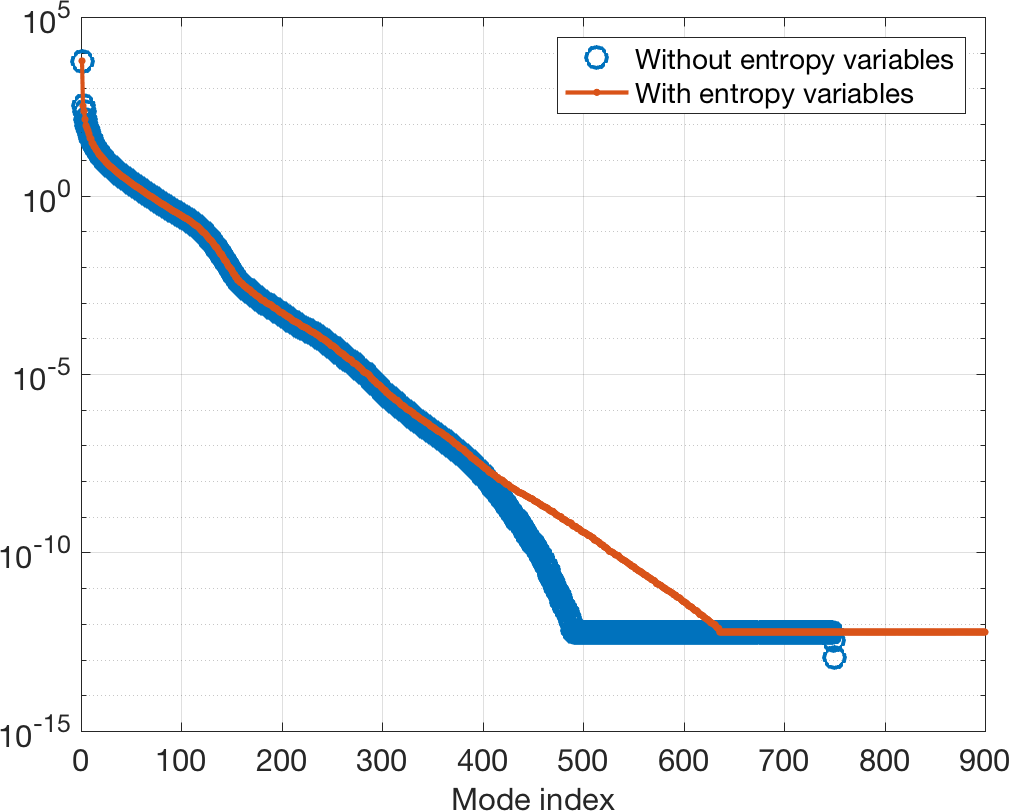
\includegraphics[width=.33\textwidth]{UVsingularvalues.png}}\label{subfig:a}}
\hspace{.02em}
\subfloat[Fifth singular vector]{\raisebox{.615em}{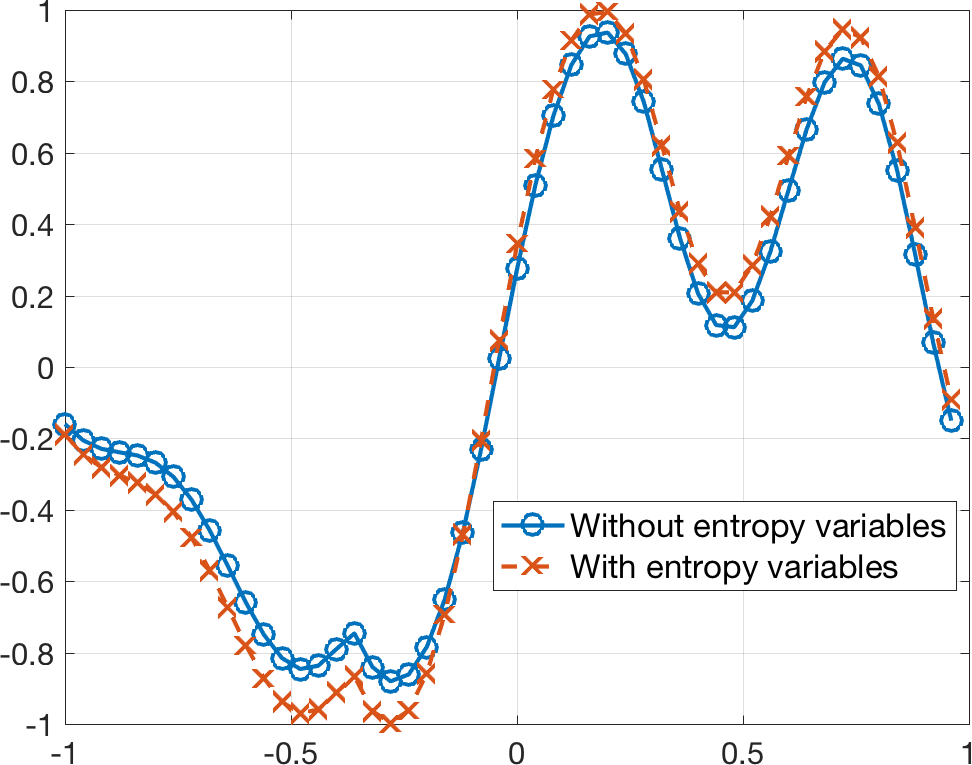
\includegraphics[width=.322\textwidth]{UVsingularvector.png}}\label{subfig:c}}
\hspace{.02em}
\subfloat[Projection errors, 25 modes]{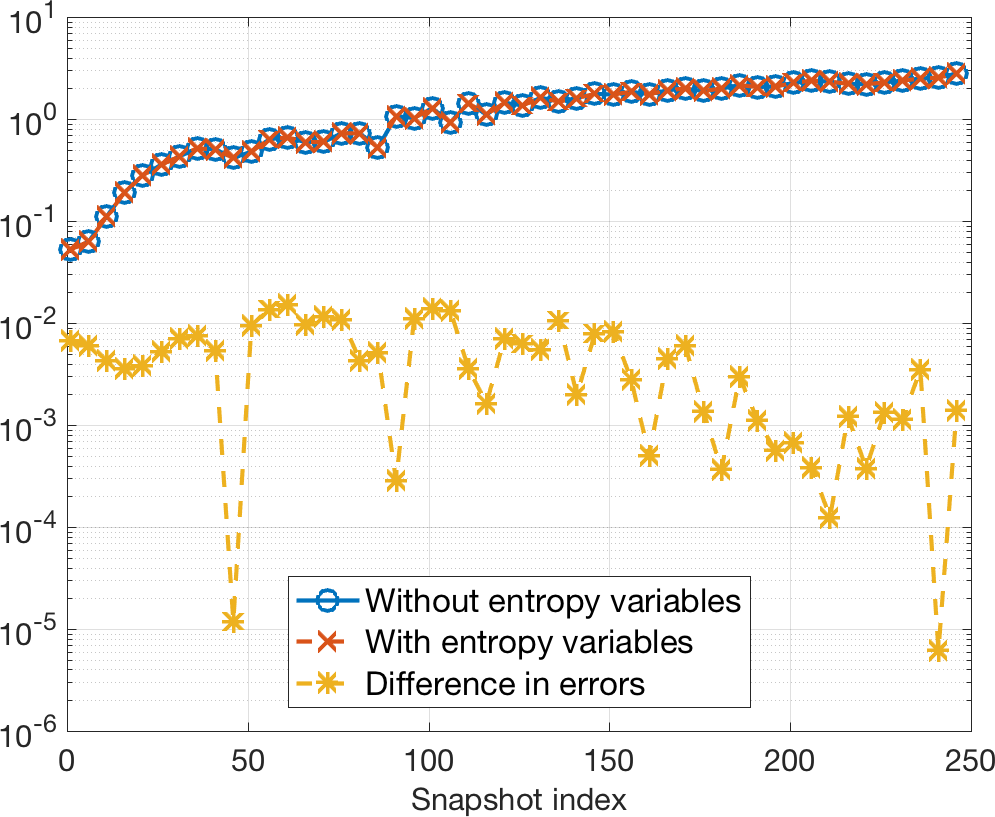
\includegraphics[width=.33\textwidth]{UVprojectionerrors.png}\label{subfig:b}}
\caption{Behavior of the SVD and reduced basis functions with and without entropy variable enrichment of the solution snapshots. }
\label{fig:svd}
\end{figure}

We next examine solutions produced by the reduced order models.  We observe that the reduced models can utilize a larger CFL; however, to ensure that temporal errors are small, all solutions are computed using the same CFL as the full order model.  Figure~\ref{fig:romsols} shows density computed using 25, 75, and 125 modes and the hyper-reduced treatment of viscosity in (\ref{eq:visc2}).  For all resolutions, the shock is under-resolved and the solution possesses Gibbs-type oscillations.  However, despite this under-resolution, the ROM remains stable and does not blow up.  In all cases, we compute hyper-reductions of both convective and viscous terms.  For 25 modes, 92 convective hyper-reduced points and 133 viscous hyper-reduced points are used.  For 75 modes, 245 convective hyper-reduced points and 242 viscous hyper-reduced points are used.  For 125 modes, 410 convective hyper-reduced points and 292 viscous hyper-reduced points are used.  
\begin{figure}
\centering
\subfloat[25 modes, $T=.25$]{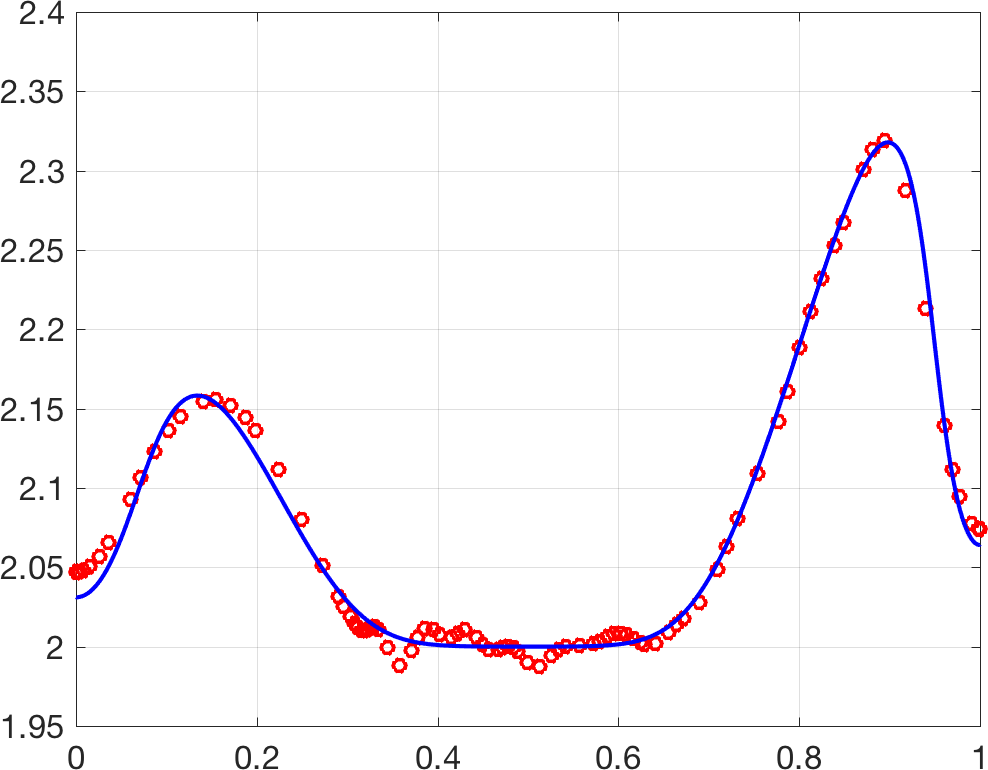
\includegraphics[width=.32\textwidth]{euler1Dwall_t25_25modes.png}}
\hspace{.05em}
\subfloat[75 modes, $T=.25$]{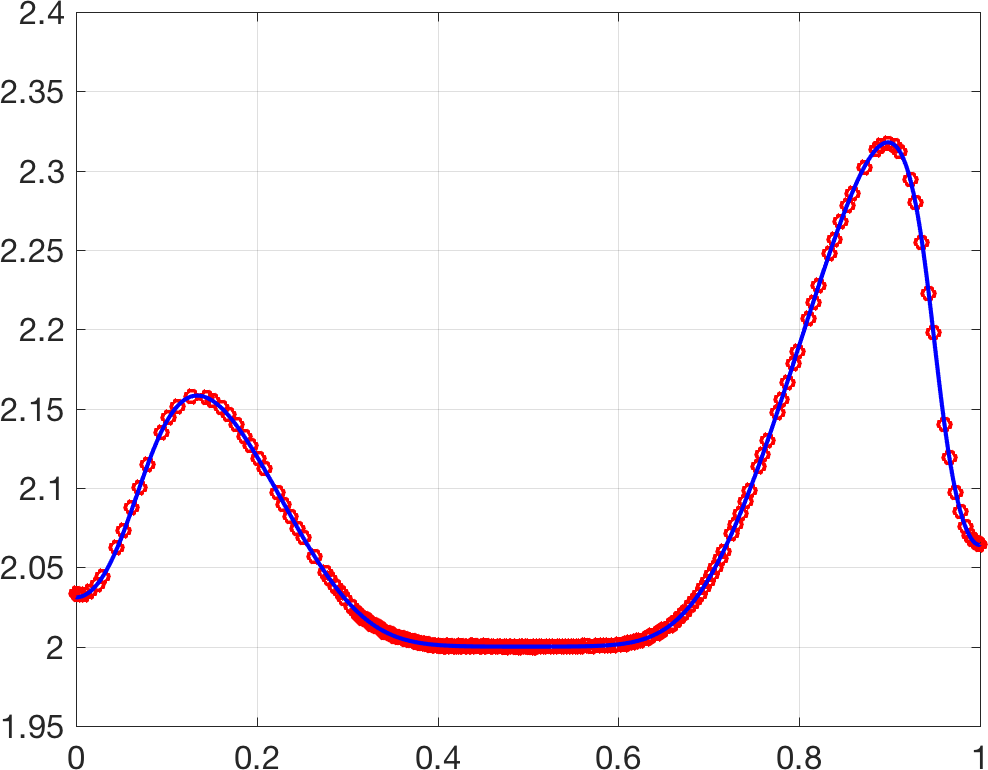
\includegraphics[width=.32\textwidth]{euler1Dwall_t25_75modes.png}}
\hspace{.05em}
\subfloat[125 modes, $T=.25$]{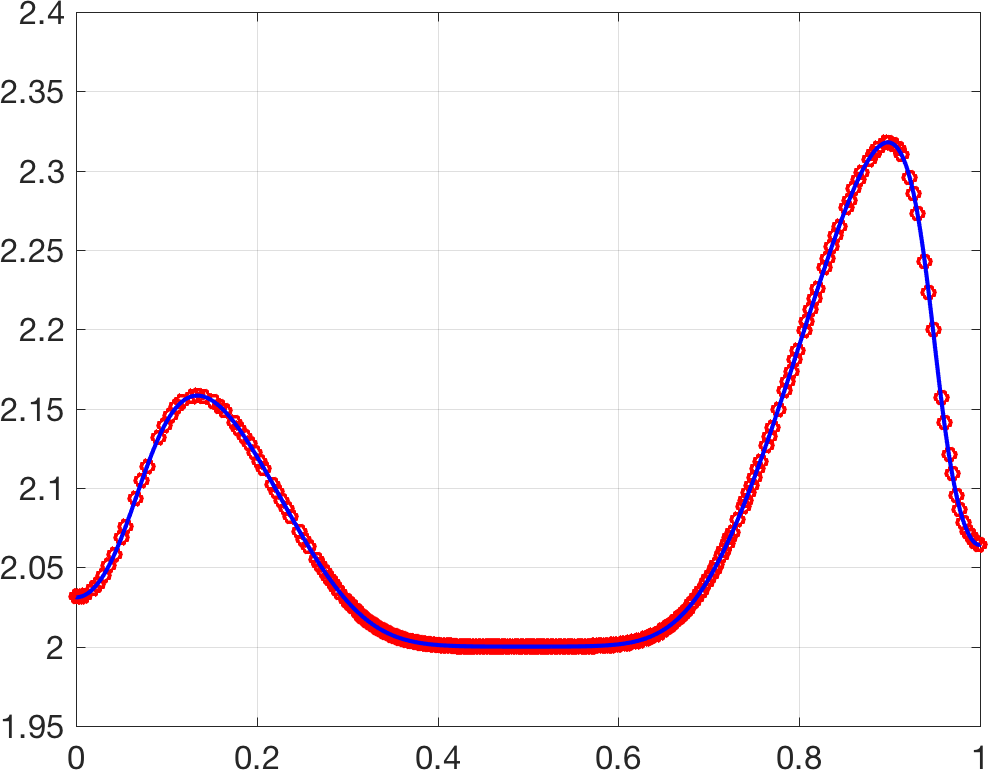
\includegraphics[width=.32\textwidth]{euler1Dwall_t25_125modes.png}}\\
\subfloat[25 modes, $T=.25$]{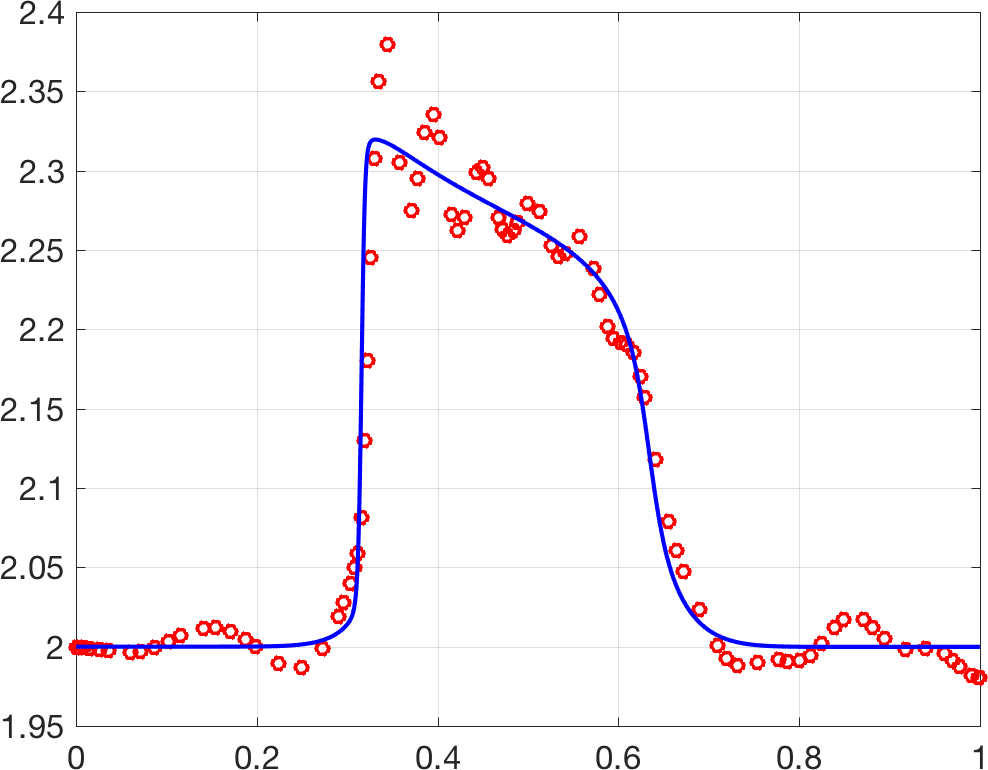
\includegraphics[width=.32\textwidth]{euler1Dwall_t75_25modes.png}}
\hspace{.05em}
\subfloat[75 modes, $T=.25$]{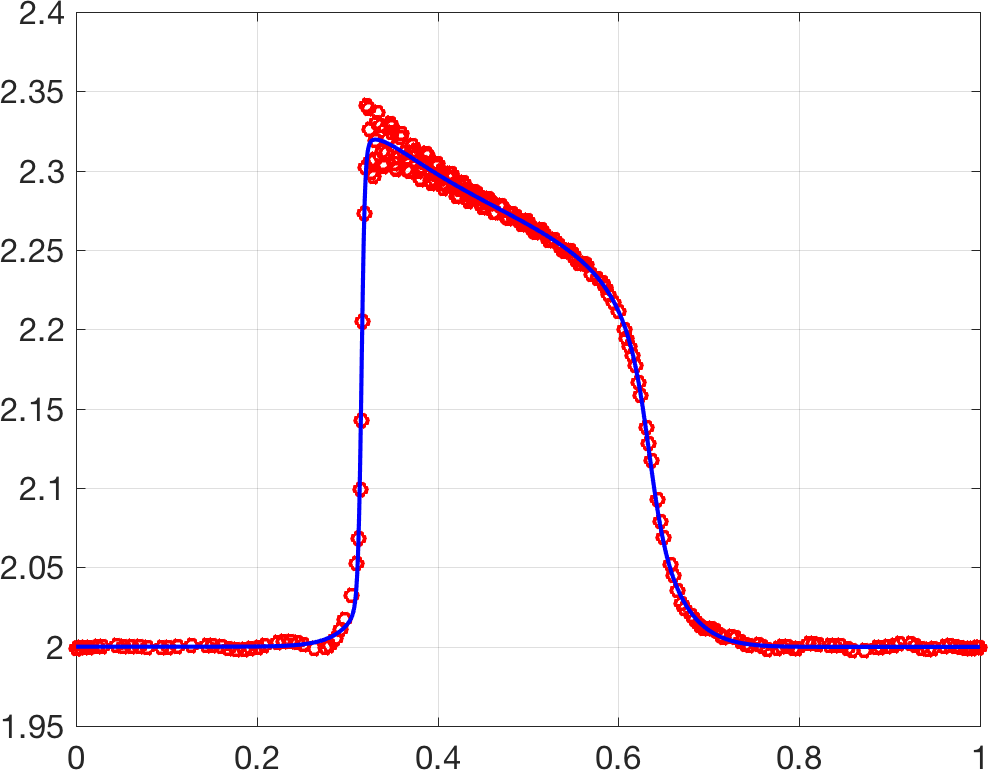
\includegraphics[width=.32\textwidth]{euler1Dwall_t75_75modes.png}}
\hspace{.05em}
\subfloat[125 modes, $T=.25$]{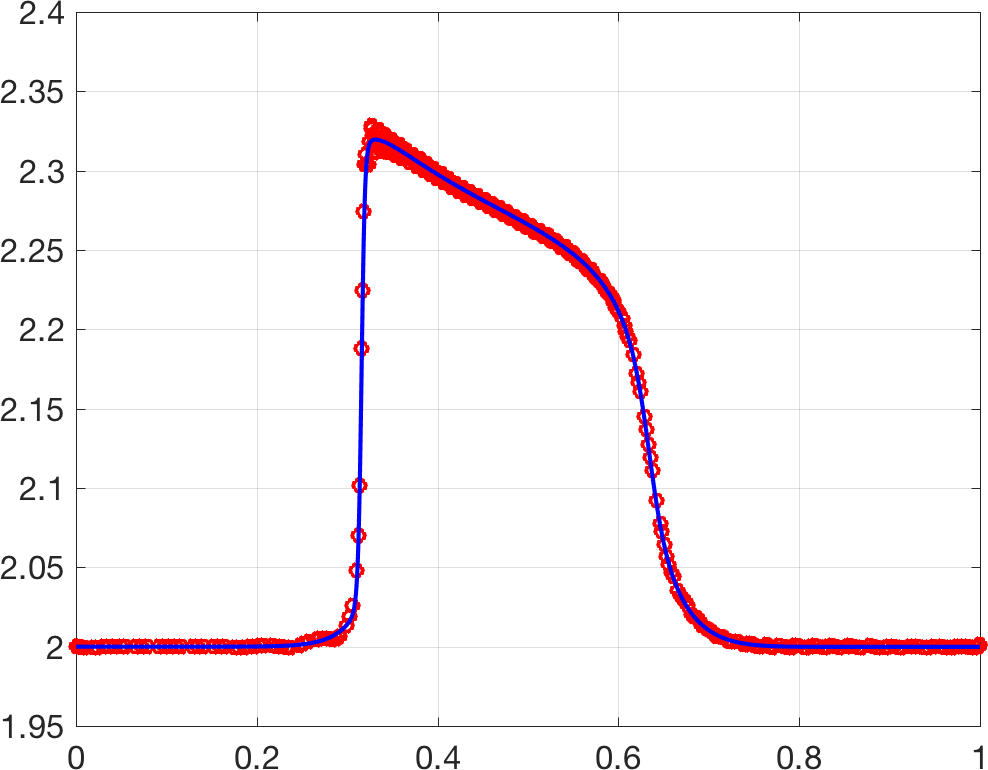
\includegraphics[width=.32\textwidth]{euler1Dwall_t75_125modes.png}}
\caption{Density $\rho$ computed using 25, 75, and 125 modes at times $T=.25, .75$.   }
\label{fig:romsols}
\end{figure}

Next, we examine the difference in the hyper-reduced treatments of entropy dissipation (\ref{eq:visc1}), (\ref{eq:visc2}), and (\ref{eq:visc3}) described in Section~\ref{sec:diss} (recall that (\ref{eq:visc3}) is not provably entropy dissipative).  We have verified that the convective term $\bm{v}_N^T \bm{V}_h^T\LRp{\bm{Q}_h \circ \bm{F}}\bm{1}$ is $O\LRp{10^{-15}}$ (near machine precision) over the entire simulation, confirming that the formulation (\ref{eq:esbchr}) is discretely entropy conservative in the absence of viscosity and boundary flux penalization terms.  Thus, if the discrete entropy dissipation $\bm{v}_N^T\bm{d}(\bm{u}_N)$ is positive, then the simulation is entropy stable.  Figure~\ref{fig:entropydiss}  shows the computed entropy dissipation over the time interval $[0,.75]$.  All hyper-reduced treatments produce similar results, with the entropy dissipation produced by the naive approximation (\ref{eq:visc3}) differing most significantly.  The naive approximation differs from (\ref{eq:visc1}) and (\ref{eq:visc2}) by about $O\LRp{10^{-1}}$ to $O\LRp{10^{-2}}$, while (\ref{eq:visc1}) differs from (\ref{eq:visc2}) by $O\LRp{10^{-6}}$.  
\begin{figure}
\centering
\subfloat[25 modes]{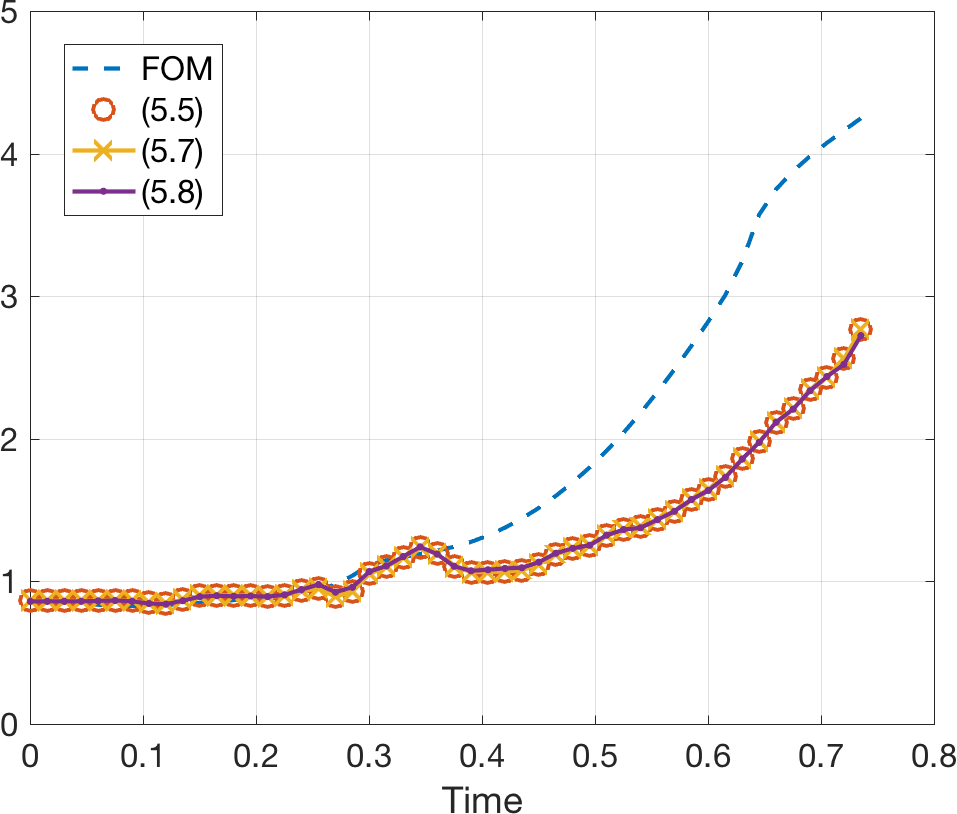
\includegraphics[width=.45\textwidth]{visc25modes.png}}
\hspace{.5em}
%\subfloat[Difference, 25 modes]{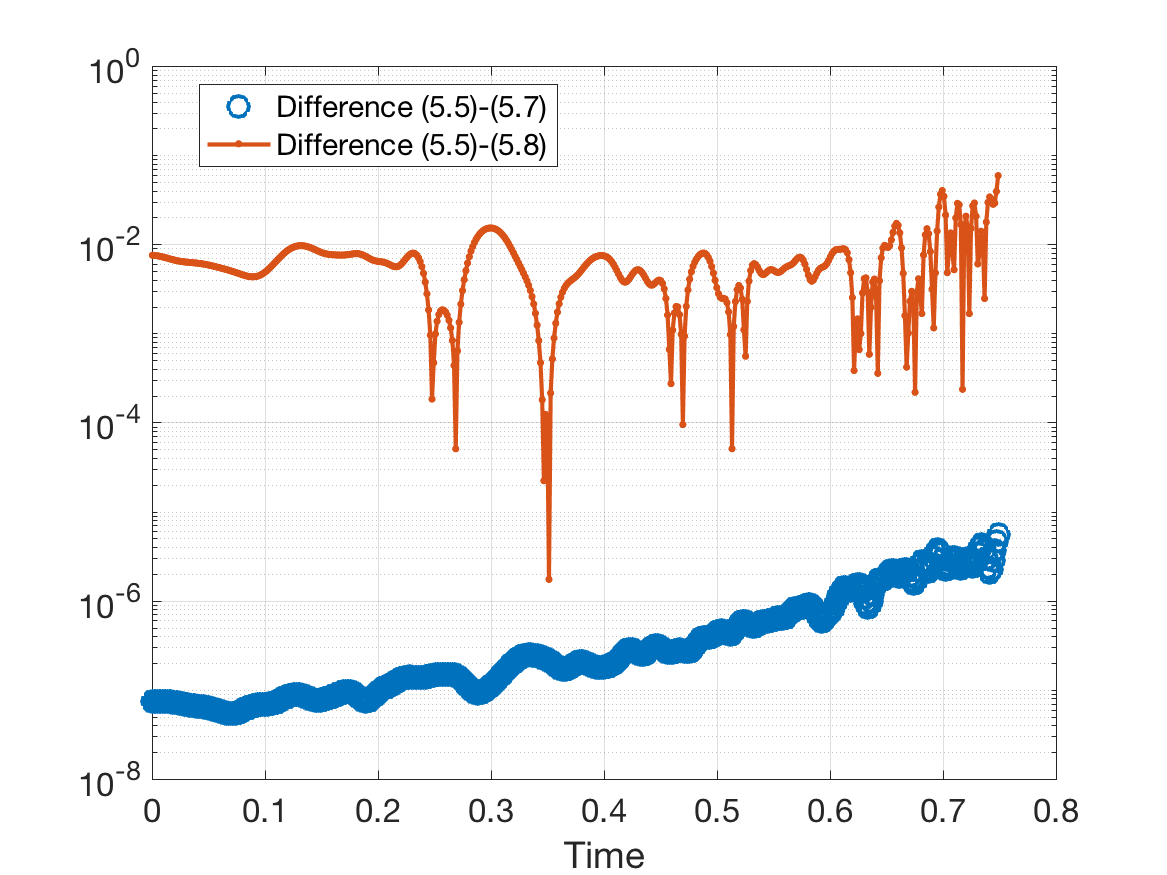
\includegraphics[width=.32\textwidth]{viscdiff25modes.png}}
\subfloat[75 modes]{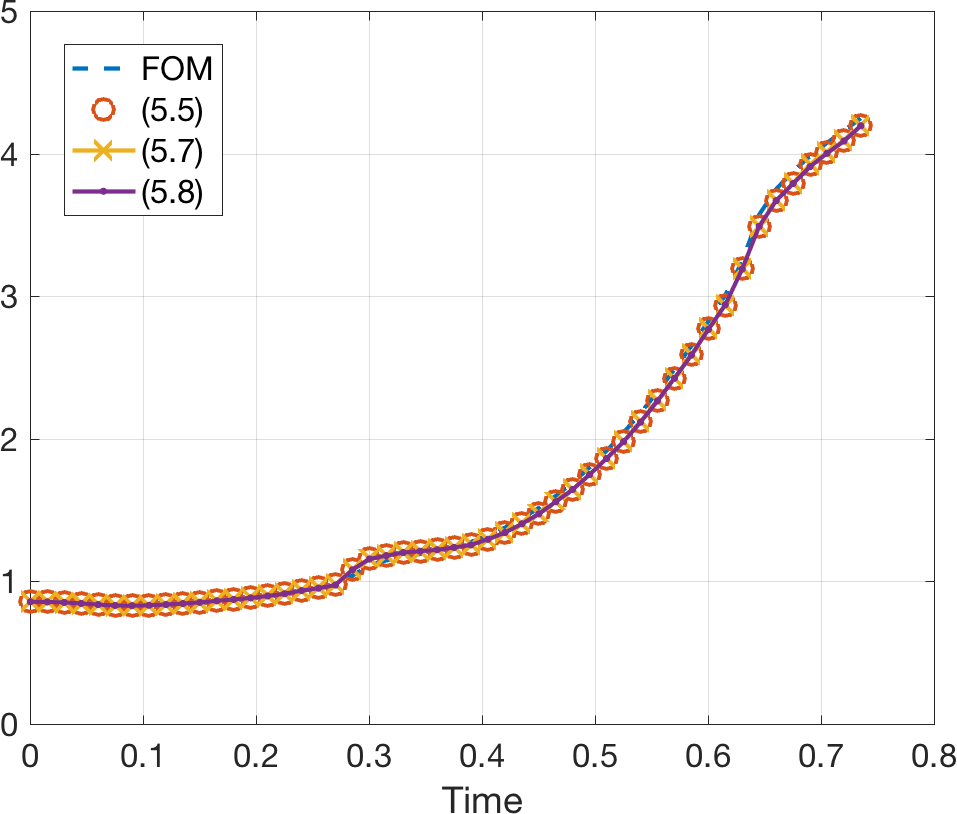
\includegraphics[width=.45\textwidth]{visc75modes.png}}
\caption{Discrete entropy dissipation $\bm{v}_N^T\bm{d}(\bm{u}_N)$ computed using (\ref{eq:visc1}), (\ref{eq:visc2}), and (\ref{eq:visc3}) for 25 and 75 modes.}
\label{fig:entropydiss}
\end{figure}

We now compare the evolution of errors and entropy, and examine the effect of hyper-reduction on the discrete solution in Figure~\ref{fig:entropyevo}.  We observe that the evolution of the ROM average discrete entropy converges to the average discrete entropy for the full order model as the number of modes increases from 25 to 75.  For 125 modes, the average entropies for the ROM and FOM are indistinguishable.  The errors behave similarly, decreasing as the number of modes increases.  For reference, we also include errors computed without hyper-reduction using (\ref{eq:esrom}).  We observe that the hyper-reduced errors are similar to errors without hyper-reduction in all cases, though for $75$ modes, hyper-reduction produces lower errors.  The reasons for this are unclear.
\begin{figure}
\centering
\subfloat[Evolution of entropy]{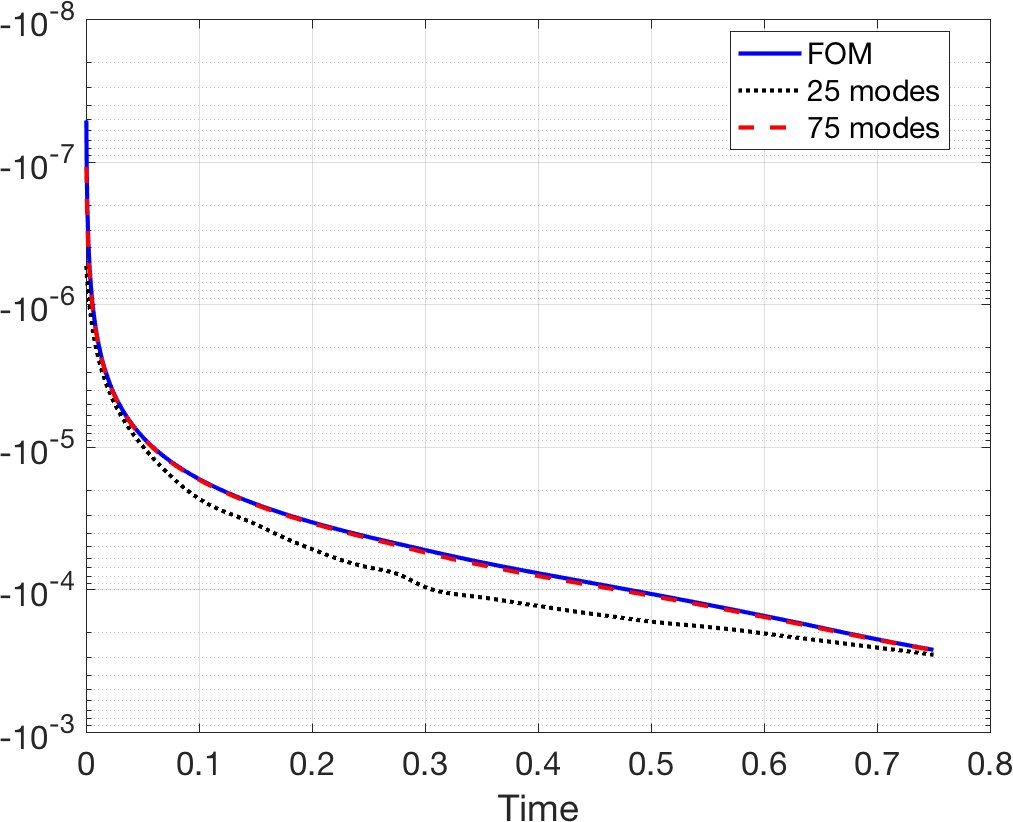
\includegraphics[height=.24\textheight]{entropyevolution.png}}
\hspace{.5em}
\subfloat[Error between ROM and FOM]{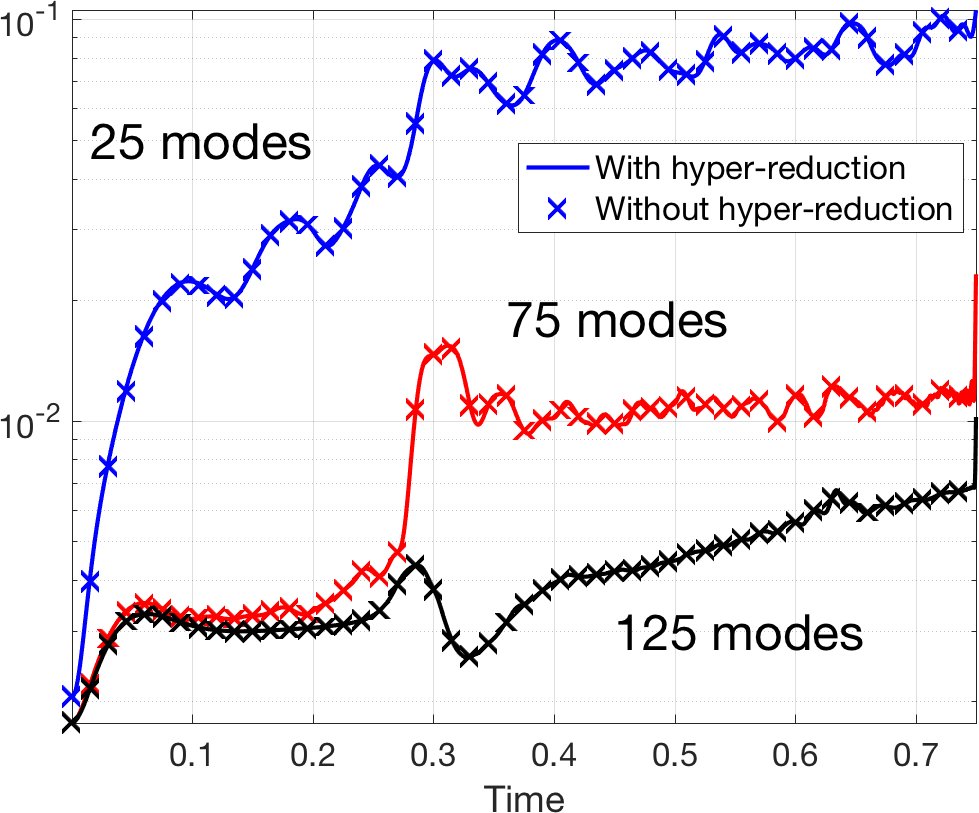
\includegraphics[height=.235\textheight]{euler_error_hypred_comparison_K2500}}
%\hspace{.1em}
%\subfloat[Difference, 25 modes]{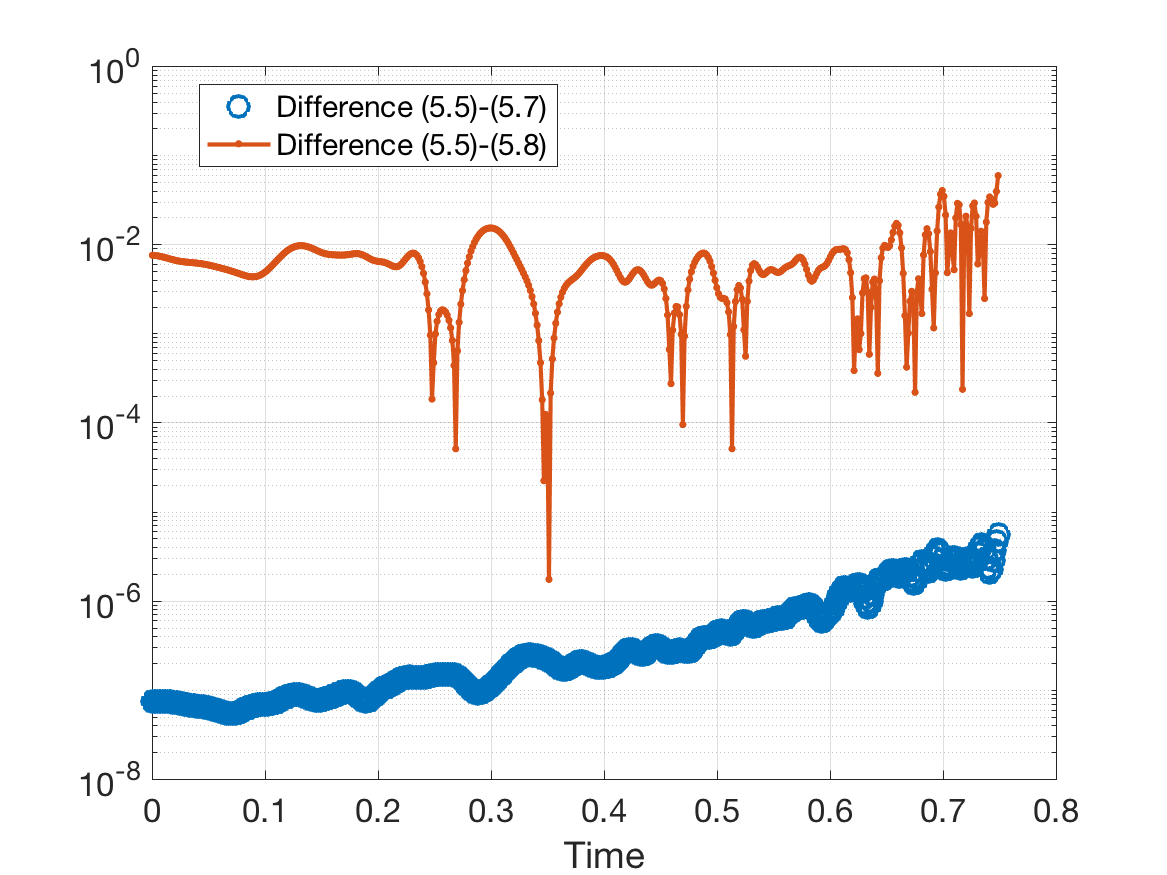
\includegraphics[width=.32\textwidth]{viscdiff25modes.png}}
%\subfloat[Entropy 75 modes]{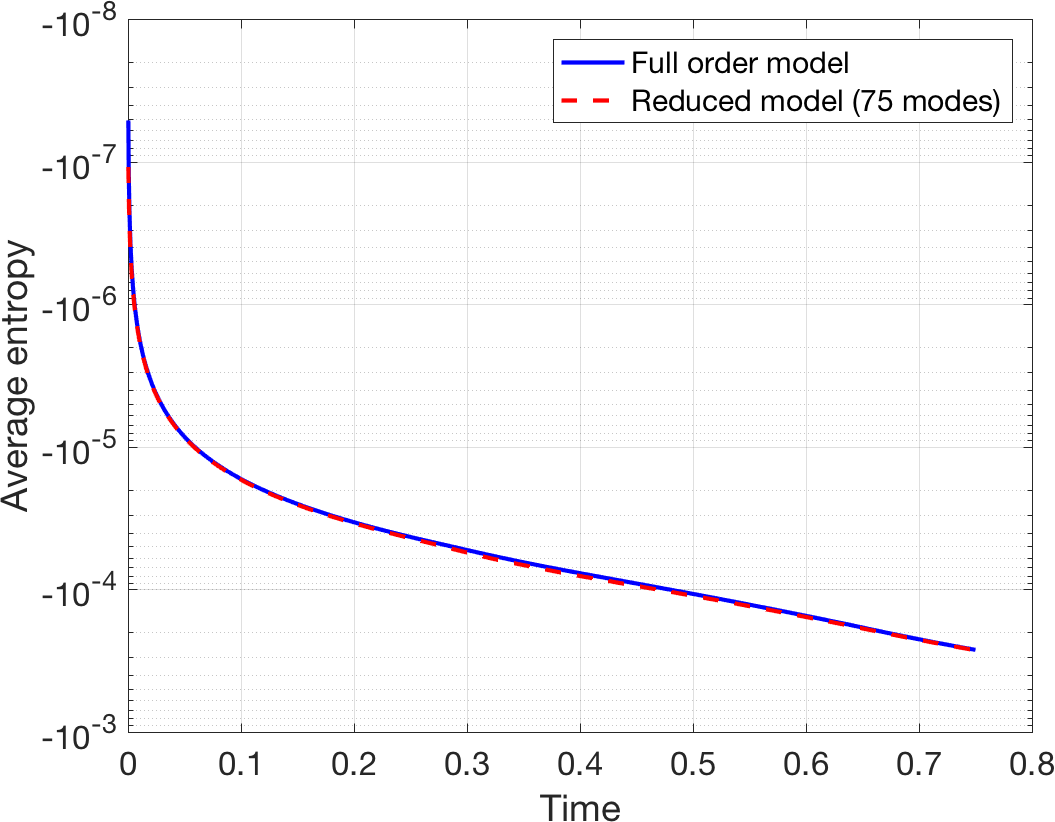
\includegraphics[width=.32\textwidth]{euler1Dwall_entropy_75modes.png}}
\caption{Evolution of error (with and without hyper-reduction) and entropy over time interval $[0,.75]$ for $25, 75, 125$ modes.}
\label{fig:entropyevo}
\end{figure}

%Next, we examine 

%\subsection{1D Euler equations with wall boundary conditions}
%\subsection{Accuracy of entropy projection}

%\subsection{2D periodic Euler equations}

\subsection{2D Euler equations}% with wall boundary conditions}

We now study the Euler equations in 2D with wall boundary conditions.  It was shown in \cite{svard2014entropy, chen2017entropy} that wall boundary conditions can be imposed using a ``mirror state''.  Let $\bm{n}$ denote the outward normal at a wall, and let $\bm{u}_{\bm{n}} = un_x + vn_y$ and $\bm{u}_{\bm{n}^\perp} = un_y - vn_x$ denote the normal and tangential components of the velocity at the wall.  We use a boundary numerical flux $\bm{f}^* = \bm{f}_S\LRp{\bm{u}^+,\bm{u}}$ augmented with local Lax-Friedrichs penalization, where the exterior state $\bm{u}^+$ is defined by
\[
\rho^+ = \rho, \qquad \bm{u}_{\bm{n}}^+ = -\bm{u}_{\bm{n}}, \qquad \bm{u}_{\bm{n}^\perp}^+ = \bm{u}_{\bm{n}^\perp}, \qquad p^+ = p.  
\]
We set a Gaussian pulse initial condition 
\[
\rho = 1 + e^{-50\LRp{x^2+(y+1/2)^2}}, \qquad \bm{u} = \bm{0}, \qquad p = \rho^{\gamma}.  
\]
The full order model is computed on a $100\times 100$ grid with viscosity coefficient $\epsilon = 1e-3$, and the reduced order solution is shown in Figure~\ref{fig:pulse2d}. Since little difference is observed between the hyper-reducted treatments of viscosity,  the naive treatment (\ref{eq:visc3}) is used.  The solution does not form shock disccontinuities, and is chosen instead to test the imposition of boundary conditions.  We note that, due to the nature of the linear programming software used to compute the boundary weights, the constraints (\ref{eq:sbpconstraints}) on the boundary weights $\bm{w}_b$ are imposed to a tolerance of $5e-8$.  Despite this inexact enforcement of constraints, the computed entropy RHS remained small, oscillating around $10^{-11}$ in the absence of entropy dissipative terms.  

\begin{figure}
\centering
\subfloat[Full order model]{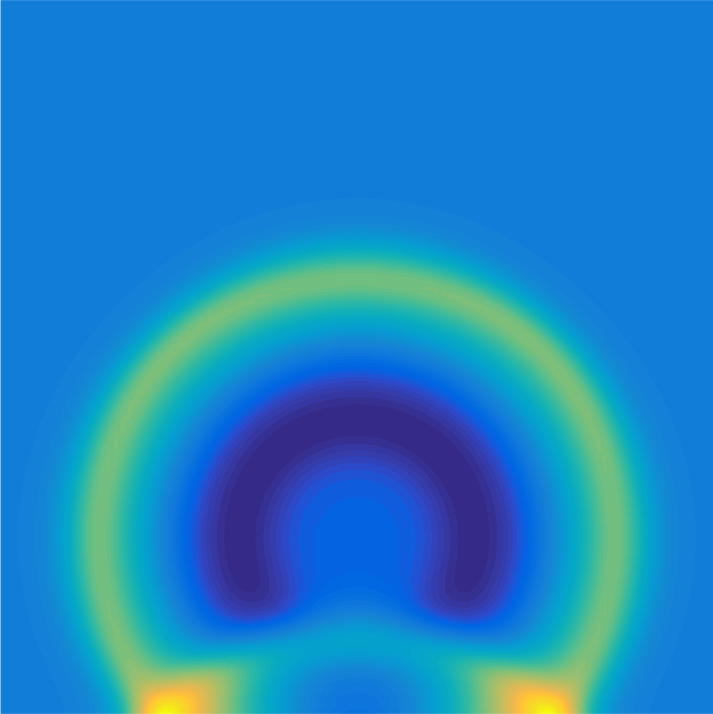
\includegraphics[width=.32\textwidth]{pulse2d.png}}
\hspace{.1em}
\subfloat[Reduced order model]{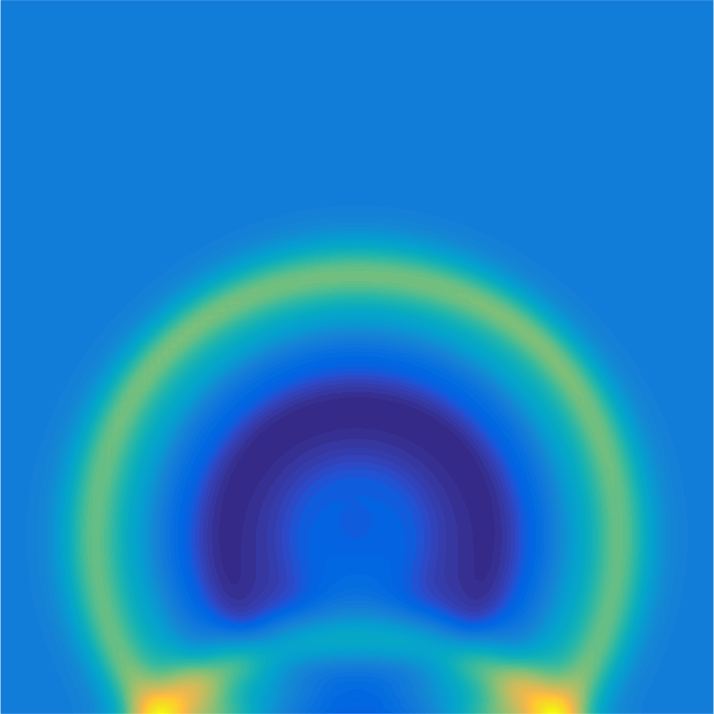
\includegraphics[width=.32\textwidth]{pulse2d_ROM.png}}
\hspace{.1em}
\subfloat[Hyper-reduction points]{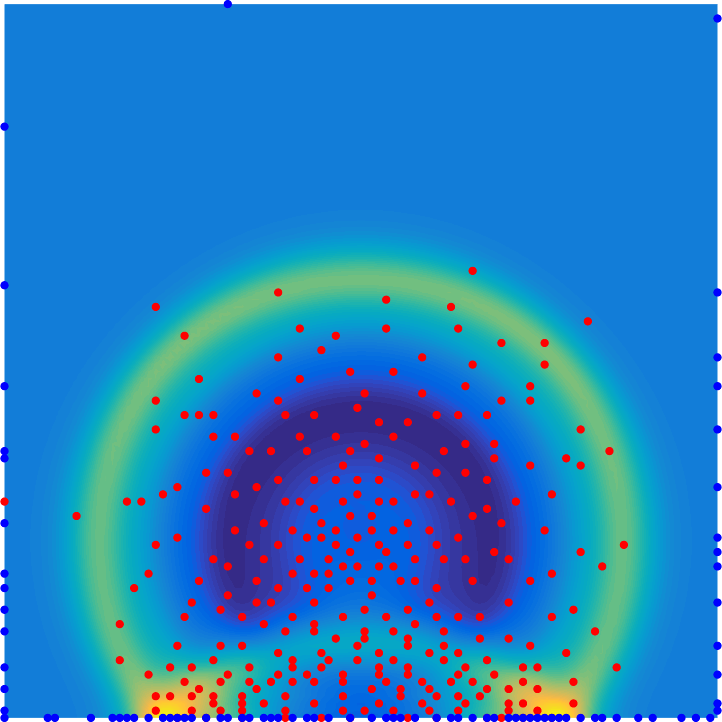
\includegraphics[width=.32\textwidth]{pulse2d_ROM_pts.png}}
\caption{Density computed using 25 modes, 303 hyper-reduced volume points, and 75 hyper-reduced boundary points.  The relative $L^2$ error is $.00934$.}
\label{fig:pulse2d}
\end{figure}

\section{Conclusion}

\section{Acknowledgments}

The author thanks Matthias Heinkenschloss, Matthew Zahr, and Masayuki Yano for informative discussions.

\bibliographystyle{unsrt}
\bibliography{refs}



\end{document}


